\ifx\master\undefined% AUTOCOMPILE
% Allows for individual chapters to be compiled.

% Usage:
% \ifx\master\undefined% AUTOCOMPILE
% Allows for individual chapters to be compiled.

% Usage:
% \ifx\master\undefined% AUTOCOMPILE
% Allows for individual chapters to be compiled.

% Usage:
% \ifx\master\undefined\input{../settings/autocompile}\fi
% (place at start and end of chapter file)

\ifx\noprelim\undefined
    % first time included
    % input preamble files
    \input{../settings/phdsetup}

    \begin{document}
    \def\noprelim{}
\else
    % already included once
    % input post files

    \singlespacing
    \bibliographystyle{../bibliography/expanded}
    \bibliography{../bibliography/references}

    \end{document}
\fi\fi
% (place at start and end of chapter file)

\ifx\noprelim\undefined
    % first time included
    % input preamble files
    % [ USER VARIABLES ]

\def\PHDTITLE {Extensions of the Theory of Computational Mechanics}
\def\PHDAUTHOR{Evan Klose Friis}
\def\PHDSCHOOL{University of California, Davis}

\def\PHDMONTH {June}
\def\PHDYEAR  {2011}
\def\PHDDEPT {Physics}

\def\BSSCHOOL {University of California at San Diego}
\def\BSYEAR   {2005}

\def\PHDCOMMITTEEA{Professor John Conway}
\def\PHDCOMMITTEEB{Professor Robin Erbacher}
\def\PHDCOMMITTEEC{Professor Mani Tripathi}

% [ GLOBAL SETUP ]

\documentclass[letterpaper,oneside,11pt]{report}

\usepackage{calc}
\usepackage{breakcites}
\usepackage[newcommands]{ragged2e}

\usepackage[pdftex]{graphicx}
\usepackage{epstopdf}

%\usepackage{tikz}
%\usetikzlibrary{positioning} % [right=of ...]
%\usetikzlibrary{fit} % [fit= ...]

%\pgfdeclarelayer{background layer}
%\pgfdeclarelayer{foreground layer}
%\pgfsetlayers{background layer,main,foreground layer}

%\newenvironment{wrap}{\noindent\begin{minipage}[t]{\linewidth}\vspace{-0.5\normalbaselineskip}\centering}{\vspace{0.5\normalbaselineskip}\end{minipage}}

%% [Venn diagram environment]
%\newenvironment{venn2}
%{\begin{tikzpicture} [every pin/.style={text=black, text opacity=1.0, pin distance=0.5cm, pin edge={black!60, semithick}},
%% define a new style 'venn'
%venn/.style={circle, draw=black!60, semithick, minimum size = 4cm}]
%
%% create circle and give it external (pin) label
%\node[venn] (X) at (-1,0) [pin={150:$H[X]$}] {};
%\node[venn] (Y) at (1,0) [pin={30:$H[Y]$}] {};
%
%% place labels of the atoms by hand
%\node at (-1.9,0) {$H[X|Y]$};
%\node at (1.9,0) {$H[Y|X]$};
%\node at (0,0) {$I[X;Y]$};}
%{\end{tikzpicture}}

%\newcommand{\wrapmath}[1]{\begin{wrap}\begin{tikzpicture}[every node/.style={inner ysep=0ex, inner xsep=0em}]\node[] {$\displaystyle\begin{aligned} #1\end{aligned}$};\end{tikzpicture}\end{wrap}}

\renewenvironment{abstract}{\chapter*{Abstract}}{}
\renewcommand{\bibname}{Bibliography}
\renewcommand{\contentsname}{Table of Contents}

\makeatletter
\renewcommand{\@biblabel}[1]{\textsc{#1}}
\makeatother

% [ FONT SETTINGS ]

\usepackage[tbtags, intlimits, namelimits]{amsmath}
\usepackage[adobe-utopia]{mathdesign}

\DeclareSymbolFont{pazomath}{OMS}{zplm}{m}{n}
\DeclareSymbolFontAlphabet{\mathcal}{pazomath}
\SetMathAlphabet\mathcal{bold}{OMS}{zplm}{b}{n}

\SetSymbolFont{largesymbols}{normal}{OMX}{zplm}{m}{n}
\SetSymbolFont{largesymbols}{bold}{OMX}{zplm}{m}{n}
\SetSymbolFont{symbols}{normal}{OMS}{zplm}{m}{n}
\SetSymbolFont{symbols}{bold}{OMS}{zplm}{b}{n}

\renewcommand{\sfdefault}{phv}
\renewcommand{\ttdefault}{fvm}

\widowpenalty 8000
\clubpenalty  8000

% [ PAGE LAYOUT ]
\usepackage{geometry}
\geometry{lmargin = 1.5in}
\geometry{rmargin = 1.0in}
\geometry{tmargin = 1.0in}
\geometry{bmargin = 1.0in}

% [ PDF SETTINGS ]

\usepackage[final]{hyperref}
\hypersetup{breaklinks  = true}
\hypersetup{colorlinks  = true}
\hypersetup{linktocpage = false}
\hypersetup{linkcolor   = blue}
\hypersetup{citecolor   = green}
\hypersetup{urlcolor    = black}
\hypersetup{plainpages  = false}
\hypersetup{pageanchor  = true}
\hypersetup{pdfauthor   = {\PHDAUTHOR}}
\hypersetup{pdftitle    = {\PHDTITLE}}
\hypersetup{pdfsubject  = {Dissertation, \PHDSCHOOL}}
\urlstyle{same}

% [ LETTER SPACING ]

\usepackage[final]{microtype}
\microtypesetup{protrusion=compatibility}
\microtypesetup{expansion=false}

\newcommand{\upper}[1]{\MakeUppercase{#1}}
\let\lsscshape\scshape

\ifcase\pdfoutput\else\microtypesetup{letterspace=15}
\renewcommand{\scshape}{\lsscshape\lsstyle}
\renewcommand{\upper}[1]{\textls[50]{\MakeUppercase{#1}}}\fi

% [ LINE SPACING ]

\usepackage[doublespacing]{setspace}
\renewcommand{\displayskipstretch}{0.0}

\setlength{\parskip   }{0em}
\setlength{\parindent }{2em}

% [ TABLE FORMATTING ]

\usepackage{booktabs}
\setlength{\heavyrulewidth}{1.5\arrayrulewidth}
\setlength{\lightrulewidth}{1.0\arrayrulewidth}
\setlength{\doublerulesep }{2.0\arrayrulewidth}

% [ SECTION FORMATTING ]

\usepackage[largestsep,nobottomtitles*]{titlesec}
\renewcommand{\bottomtitlespace}{0.75in}

\titleformat{\chapter}[display]{\bfseries\huge\singlespacing}{\filleft\textsc{\LARGE \chaptertitlename\ \thechapter}}{-0.2ex}{\titlerule[3pt]\vspace{0.2ex}}[]

\titleformat{\section}{\LARGE}{\S\thesection\hspace{0.5em}}{0ex}{}
\titleformat{\subsection}{\Large}{\S\thesubsection\hspace{0.5em}}{0ex}{}
\titleformat{\subsubsection}{\large}{\thesubsubsection\hspace{0.5em}}{0ex}{}

\titlespacing*{\chapter}{0em}{6ex}{4ex plus 2ex minus 0ex}
\titlespacing*{\section}{0em}{2ex plus 3ex minus 1ex}{0.5ex plus 0.5ex minus 0.5ex}
\titlespacing*{\subsection}{0ex}{2ex plus 3ex minus 1ex}{0ex}
\titlespacing*{\subsubsection}{0ex}{2ex plus 0ex minus 1ex}{0ex}

% [ HEADER SETTINGS ]

\usepackage{fancyhdr}

\setlength{\headheight}{\normalbaselineskip}
\setlength{\footskip  }{0.5in}
\setlength{\headsep   }{0.5in-\headheight}

\fancyheadoffset[R]{0.5in}
\renewcommand{\headrulewidth}{0pt}
\renewcommand{\footrulewidth}{0pt}

\newcommand{\pagebox}{\parbox[r][\headheight][t]{0.5in}{\hspace\fill\thepage}}

\newcommand{\prelimheaders}{\ifx\prelim\undefined\renewcommand{\thepage}{\textit{\roman{page}}}\fancypagestyle{plain}{\fancyhf{}\fancyfoot[L]{\makebox[\textwidth-0.5in]{\thepage}}}\pagestyle{plain}\def\prelim{}\fi}

\newcommand{\normalheaders}{\renewcommand{\thepage}{\arabic{page}}\fancypagestyle{plain}{\fancyhf{}\fancyhead[R]{\pagebox}}\pagestyle{plain}}

\normalheaders{}

% [ CUSTOM COMMANDS ]

\newcommand{\signaturebox}[1]{\multicolumn{1}{p{4in}}{\vspace{3ex}}\\\midrule #1\\}

%\input{../includes/cmechabbrev}

% [some math stuff - maybe stick in sep file]
\usepackage{amsthm}
\usepackage{amscd}
\theoremstyle{plain}    \newtheorem{Lem}{Lemma}
\theoremstyle{plain}    \newtheorem*{ProLem}{Proof}
\theoremstyle{plain} 	\newtheorem{Cor}{Corollary}
\theoremstyle{plain} 	\newtheorem*{ProCor}{Proof}
\theoremstyle{plain} 	\newtheorem{The}{Theorem}
\theoremstyle{plain} 	\newtheorem*{ProThe}{Proof}
\theoremstyle{plain} 	\newtheorem{Prop}{Proposition}
\theoremstyle{plain} 	\newtheorem*{ProProp}{Proof}
\theoremstyle{plain} 	\newtheorem*{Conj}{Conjecture}
\theoremstyle{plain}	\newtheorem*{Rem}{Remark}
\theoremstyle{plain}	\newtheorem*{Def}{Definition} 
\theoremstyle{plain}	\newtheorem*{Not}{Notation}

% [uniform figure scaling - maybe this is not a good idea]
\def\figscale{.7}
\def\lscale{1.0}

% [FIX ME! - red makes it easier to spot]
\newcommand{\FIX}[1]{\textbf{\textcolor{red}{#1}}}


    \begin{document}
    \def\noprelim{}
\else
    % already included once
    % input post files

    \singlespacing
    \bibliographystyle{../bibliography/expanded}
    \bibliography{../bibliography/references}

    \end{document}
\fi\fi
% (place at start and end of chapter file)

\ifx\noprelim\undefined
    % first time included
    % input preamble files
    % [ USER VARIABLES ]

\def\PHDTITLE {Extensions of the Theory of Computational Mechanics}
\def\PHDAUTHOR{Evan Klose Friis}
\def\PHDSCHOOL{University of California, Davis}

\def\PHDMONTH {June}
\def\PHDYEAR  {2011}
\def\PHDDEPT {Physics}

\def\BSSCHOOL {University of California at San Diego}
\def\BSYEAR   {2005}

\def\PHDCOMMITTEEA{Professor John Conway}
\def\PHDCOMMITTEEB{Professor Robin Erbacher}
\def\PHDCOMMITTEEC{Professor Mani Tripathi}

% [ GLOBAL SETUP ]

\documentclass[letterpaper,oneside,11pt]{report}

\usepackage{calc}
\usepackage{breakcites}
\usepackage[newcommands]{ragged2e}

\usepackage[pdftex]{graphicx}
\usepackage{epstopdf}

%\usepackage{tikz}
%\usetikzlibrary{positioning} % [right=of ...]
%\usetikzlibrary{fit} % [fit= ...]

%\pgfdeclarelayer{background layer}
%\pgfdeclarelayer{foreground layer}
%\pgfsetlayers{background layer,main,foreground layer}

%\newenvironment{wrap}{\noindent\begin{minipage}[t]{\linewidth}\vspace{-0.5\normalbaselineskip}\centering}{\vspace{0.5\normalbaselineskip}\end{minipage}}

%% [Venn diagram environment]
%\newenvironment{venn2}
%{\begin{tikzpicture} [every pin/.style={text=black, text opacity=1.0, pin distance=0.5cm, pin edge={black!60, semithick}},
%% define a new style 'venn'
%venn/.style={circle, draw=black!60, semithick, minimum size = 4cm}]
%
%% create circle and give it external (pin) label
%\node[venn] (X) at (-1,0) [pin={150:$H[X]$}] {};
%\node[venn] (Y) at (1,0) [pin={30:$H[Y]$}] {};
%
%% place labels of the atoms by hand
%\node at (-1.9,0) {$H[X|Y]$};
%\node at (1.9,0) {$H[Y|X]$};
%\node at (0,0) {$I[X;Y]$};}
%{\end{tikzpicture}}

%\newcommand{\wrapmath}[1]{\begin{wrap}\begin{tikzpicture}[every node/.style={inner ysep=0ex, inner xsep=0em}]\node[] {$\displaystyle\begin{aligned} #1\end{aligned}$};\end{tikzpicture}\end{wrap}}

\renewenvironment{abstract}{\chapter*{Abstract}}{}
\renewcommand{\bibname}{Bibliography}
\renewcommand{\contentsname}{Table of Contents}

\makeatletter
\renewcommand{\@biblabel}[1]{\textsc{#1}}
\makeatother

% [ FONT SETTINGS ]

\usepackage[tbtags, intlimits, namelimits]{amsmath}
\usepackage[adobe-utopia]{mathdesign}

\DeclareSymbolFont{pazomath}{OMS}{zplm}{m}{n}
\DeclareSymbolFontAlphabet{\mathcal}{pazomath}
\SetMathAlphabet\mathcal{bold}{OMS}{zplm}{b}{n}

\SetSymbolFont{largesymbols}{normal}{OMX}{zplm}{m}{n}
\SetSymbolFont{largesymbols}{bold}{OMX}{zplm}{m}{n}
\SetSymbolFont{symbols}{normal}{OMS}{zplm}{m}{n}
\SetSymbolFont{symbols}{bold}{OMS}{zplm}{b}{n}

\renewcommand{\sfdefault}{phv}
\renewcommand{\ttdefault}{fvm}

\widowpenalty 8000
\clubpenalty  8000

% [ PAGE LAYOUT ]
\usepackage{geometry}
\geometry{lmargin = 1.5in}
\geometry{rmargin = 1.0in}
\geometry{tmargin = 1.0in}
\geometry{bmargin = 1.0in}

% [ PDF SETTINGS ]

\usepackage[final]{hyperref}
\hypersetup{breaklinks  = true}
\hypersetup{colorlinks  = true}
\hypersetup{linktocpage = false}
\hypersetup{linkcolor   = blue}
\hypersetup{citecolor   = green}
\hypersetup{urlcolor    = black}
\hypersetup{plainpages  = false}
\hypersetup{pageanchor  = true}
\hypersetup{pdfauthor   = {\PHDAUTHOR}}
\hypersetup{pdftitle    = {\PHDTITLE}}
\hypersetup{pdfsubject  = {Dissertation, \PHDSCHOOL}}
\urlstyle{same}

% [ LETTER SPACING ]

\usepackage[final]{microtype}
\microtypesetup{protrusion=compatibility}
\microtypesetup{expansion=false}

\newcommand{\upper}[1]{\MakeUppercase{#1}}
\let\lsscshape\scshape

\ifcase\pdfoutput\else\microtypesetup{letterspace=15}
\renewcommand{\scshape}{\lsscshape\lsstyle}
\renewcommand{\upper}[1]{\textls[50]{\MakeUppercase{#1}}}\fi

% [ LINE SPACING ]

\usepackage[doublespacing]{setspace}
\renewcommand{\displayskipstretch}{0.0}

\setlength{\parskip   }{0em}
\setlength{\parindent }{2em}

% [ TABLE FORMATTING ]

\usepackage{booktabs}
\setlength{\heavyrulewidth}{1.5\arrayrulewidth}
\setlength{\lightrulewidth}{1.0\arrayrulewidth}
\setlength{\doublerulesep }{2.0\arrayrulewidth}

% [ SECTION FORMATTING ]

\usepackage[largestsep,nobottomtitles*]{titlesec}
\renewcommand{\bottomtitlespace}{0.75in}

\titleformat{\chapter}[display]{\bfseries\huge\singlespacing}{\filleft\textsc{\LARGE \chaptertitlename\ \thechapter}}{-0.2ex}{\titlerule[3pt]\vspace{0.2ex}}[]

\titleformat{\section}{\LARGE}{\S\thesection\hspace{0.5em}}{0ex}{}
\titleformat{\subsection}{\Large}{\S\thesubsection\hspace{0.5em}}{0ex}{}
\titleformat{\subsubsection}{\large}{\thesubsubsection\hspace{0.5em}}{0ex}{}

\titlespacing*{\chapter}{0em}{6ex}{4ex plus 2ex minus 0ex}
\titlespacing*{\section}{0em}{2ex plus 3ex minus 1ex}{0.5ex plus 0.5ex minus 0.5ex}
\titlespacing*{\subsection}{0ex}{2ex plus 3ex minus 1ex}{0ex}
\titlespacing*{\subsubsection}{0ex}{2ex plus 0ex minus 1ex}{0ex}

% [ HEADER SETTINGS ]

\usepackage{fancyhdr}

\setlength{\headheight}{\normalbaselineskip}
\setlength{\footskip  }{0.5in}
\setlength{\headsep   }{0.5in-\headheight}

\fancyheadoffset[R]{0.5in}
\renewcommand{\headrulewidth}{0pt}
\renewcommand{\footrulewidth}{0pt}

\newcommand{\pagebox}{\parbox[r][\headheight][t]{0.5in}{\hspace\fill\thepage}}

\newcommand{\prelimheaders}{\ifx\prelim\undefined\renewcommand{\thepage}{\textit{\roman{page}}}\fancypagestyle{plain}{\fancyhf{}\fancyfoot[L]{\makebox[\textwidth-0.5in]{\thepage}}}\pagestyle{plain}\def\prelim{}\fi}

\newcommand{\normalheaders}{\renewcommand{\thepage}{\arabic{page}}\fancypagestyle{plain}{\fancyhf{}\fancyhead[R]{\pagebox}}\pagestyle{plain}}

\normalheaders{}

% [ CUSTOM COMMANDS ]

\newcommand{\signaturebox}[1]{\multicolumn{1}{p{4in}}{\vspace{3ex}}\\\midrule #1\\}

%%%% macros fro standard references
%\eqref provided by amsmath
\newcommand{\figref}[1]{Fig.~\ref{#1}}
\newcommand{\tableref}[1]{Table~\ref{#1}}
\newcommand{\refcite}[1]{Ref.~\cite{#1}}

% Abbreviations from CMPPSS:

\newcommand{\eM}     {\mbox{$\epsilon$-machine}}
\newcommand{\eMs}    {\mbox{$\epsilon$-machines}}
\newcommand{\EM}     {\mbox{$\epsilon$-Machine}}
\newcommand{\EMs}    {\mbox{$\epsilon$-Machines}}
\newcommand{\eT}     {\mbox{$\epsilon$-transducer}}
\newcommand{\eTs}    {\mbox{$\epsilon$-transducers}}
\newcommand{\ET}     {\mbox{$\epsilon$-Transducer}}
\newcommand{\ETs}    {\mbox{$\epsilon$-Transducers}}

% Processes and sequences

\newcommand{\Process}{\mathcal{P}}

\newcommand{\ProbMach}{\Prob_{\mathrm{M}}}
\newcommand{\Lmax}   { {L_{\mathrm{max}}}}
\newcommand{\MeasAlphabet}	{\mathcal{A}}
% Original
%\newcommand{\MeasSymbol}   { {S} }
%\newcommand{\meassymbol}   { {s} }
% New symbol
\newcommand{\MeasSymbol}   { {X} }
\newcommand{\meassymbol}   { {x} }
\newcommand{\BiInfinity}	{ \overleftrightarrow {\MeasSymbol} }
\newcommand{\biinfinity}	{ \overleftrightarrow {\meassymbol} }
\newcommand{\Past}	{ \overleftarrow {\MeasSymbol} }
\newcommand{\past}	{ {\overleftarrow {\meassymbol}} }
\newcommand{\pastprime}	{ {\past}^{\prime}}
\newcommand{\Future}	{ \overrightarrow{\MeasSymbol} }
\newcommand{\future}	{ \overrightarrow{\meassymbol} }
\newcommand{\futureprime}	{ {\future}^{\prime}}
\newcommand{\PastPrime}	{ {\Past}^{\prime}}
\newcommand{\FuturePrime}	{ {\overrightarrow{\meassymbol}}^\prime }
\newcommand{\PastDblPrime}	{ {\overleftarrow{\meassymbol}}^{\prime\prime} }
\newcommand{\FutureDblPrime}	{ {\overrightarrow{\meassymbol}}^{\prime\prime} }
\newcommand{\pastL}	{ {\overleftarrow {\meassymbol}}{}^L }
\newcommand{\PastL}	{ {\overleftarrow {\MeasSymbol}}{}^L }
\newcommand{\PastLt}	{ {\overleftarrow {\MeasSymbol}}_t^L }
\newcommand{\PastLLessOne}	{ {\overleftarrow {\MeasSymbol}}^{L-1} }
\newcommand{\futureL}	{ {\overrightarrow{\meassymbol}}{}^L }
\newcommand{\FutureL}	{ {\overrightarrow{\MeasSymbol}}{}^L }
\newcommand{\FutureLt}	{ {\overrightarrow{\MeasSymbol}}_t^L }
\newcommand{\FutureLLessOne}	{ {\overrightarrow{\MeasSymbol}}^{L-1} }
\newcommand{\pastLprime}	{ {\overleftarrow {\meassymbol}}^{L^\prime} }
\newcommand{\futureLprime}	{ {\overrightarrow{\meassymbol}}^{L^\prime} }
\newcommand{\AllPasts}	{ { \overleftarrow {\rm {\bf \MeasSymbol}} } }
\newcommand{\AllFutures}	{ \overrightarrow {\rm {\bf \MeasSymbol}} }
\newcommand{\FutureSet}	{ \overrightarrow{\bf \MeasSymbol}}

% Causal states and epsilon-machines
\newcommand{\CausalState}	{ \mathcal{S} }
\newcommand{\CausalStatePrime}	{ {\CausalState}^{\prime}}
\newcommand{\causalstate}	{ \sigma }
\newcommand{\CausalStateSet}	{ \boldsymbol{\CausalState} }
\newcommand{\AlternateState}	{ \mathcal{R} }
\newcommand{\AlternateStatePrime}	{ {\cal R}^{\prime} }
\newcommand{\alternatestate}	{ \rho }
\newcommand{\alternatestateprime}	{ {\rho^{\prime}} }
\newcommand{\AlternateStateSet}	{ \boldsymbol{\AlternateState} }
\newcommand{\PrescientState}	{ \widehat{\AlternateState} }
\newcommand{\prescientstate}	{ \widehat{\alternatestate} }
\newcommand{\PrescientStateSet}	{ \boldsymbol{\PrescientState}}
\newcommand{\CausalEquivalence}	{ {\sim}_{\epsilon} }
\newcommand{\CausalEquivalenceNot}	{ {\not \sim}_{\epsilon}}

\newcommand{\NonCausalEquivalence}	{ {\sim}_{\eta} }
\newcommand{\NextObservable}	{ {\overrightarrow {\MeasSymbol}}^1 }
\newcommand{\LastObservable}	{ {\overleftarrow {\MeasSymbol}}^1 }
%\newcommand{\Prob}		{ {\rm P}}
\newcommand{\Prob}      {\Pr} % use standard command
\newcommand{\ProbAnd}	{ {,\;} }
\newcommand{\LLimit}	{ {L \rightarrow \infty}}
\newcommand{\Cmu}		{C_\mu}
\newcommand{\hmu}		{h_\mu}
\newcommand{\EE}		{{\bf E}}
\newcommand{\Measurable}{{\bf \mu}}

% Process Crypticity
\newcommand{\PC}		{\chi}
\newcommand{\FuturePC}		{\PC^+}
\newcommand{\PastPC}		{\PC^-}
% Causal Irreversibility
\newcommand{\CI}		{\Xi}
\newcommand{\ReverseMap}	{r}
\newcommand{\ForwardMap}	{f}

% Abbreviations from IB:
% None that aren't already in CMPPSS

% Abbreviations from Extensive Estimation:
\newcommand{\EstCausalState}	{\widehat{\CausalState}}
\newcommand{\estcausalstate}	{\widehat{\causalstate}}
\newcommand{\EstCausalStateSet}	{\boldsymbol{\EstCausalState}}
\newcommand{\EstCausalFunc}	{\widehat{\epsilon}}
\newcommand{\EstCmu}		{\widehat{\Cmu}}
\newcommand{\PastLOne}	{{\Past}^{L+1}}
\newcommand{\pastLOne}	{{\past}^{L+1}}

% Abbreviations from $\epsilon$-Transducers:
\newcommand{\InAlphabet}	{ \mathcal{A}}
\newcommand{\insymbol}		{ a}
\newcommand{\OutAlphabet}	{ \mathcal{B}}
\newcommand{\outsymbol}		{ b}
\newcommand{\InputSimple}	{ X}
\newcommand{\inputsimple}	{ x}
\newcommand{\BottleneckVar}	{\tilde{\InputSimple}}
\newcommand{\bottleneckvar}	{\tilde{\inputsimple}}
\newcommand{\InputSpace}	{ \mathbf{\InputSimple}}
\newcommand{\InputBi}	{ \overleftrightarrow {\InputSimple} }
\newcommand{\inputbi}	{ \overleftrightarrow {\inputsimple} }
\newcommand{\InputPast}	{ \overleftarrow {\InputSimple} }
\newcommand{\inputpast}	{ \overleftarrow {\inputsimple} }
\newcommand{\InputFuture}	{ \overrightarrow {\InputSimple} }
\newcommand{\inputfuture}	{ \overrightarrow {\inputsimple} }
\newcommand{\NextInput}	{ {{\InputFuture}^{1}}}
\newcommand{\NextOutput}	{ {\OutputFuture}^{1}}
\newcommand{\OutputSimple}	{ Y}
\newcommand{\outputsimple}	{ y}
\newcommand{\OutputSpace}	{ \mathbf{\OutputSimple}}
\newcommand{\OutputBi}	{ \overleftrightarrow{\OutputSimple} }
\newcommand{\outputbi}	{ \overleftrightarrow{\outputsimple} }
\newcommand{\OutputPast}	{ \overleftarrow{\OutputSimple} }
\newcommand{\outputpast}	{ \overleftarrow{\outputsimple} }
\newcommand{\OutputFuture}	{ \overrightarrow{\OutputSimple} }
\newcommand{\outputfuture}	{ \overrightarrow{\outputsimple} }
\newcommand{\OutputL}	{ {\OutputFuture}^L}
\newcommand{\outputL}	{ {\outputfuture}^L}
\newcommand{\InputLLessOne}	{ {\InputFuture}^{L-1}}
\newcommand{\inputLlessone}	{ {\inputufutre}^{L-1}}
\newcommand{\OutputPastLLessOne}	{{\OutputPast}^{L-1}_{-1}}
\newcommand{\outputpastLlessone}	{{\outputpast}^{L-1}}
\newcommand{\OutputPastLessOne}	{{\OutputPast}_{-1}}
\newcommand{\outputpastlessone}	{{\outputpast}_{-1}}
\newcommand{\OutputPastL}	{{\OutputPast}^{L}}
\newcommand{\OutputLPlusOne}	{ {\OutputFuture}^{L+1}}
\newcommand{\outputLplusone}	{ {\outputfutre}^{L+1}}
\newcommand{\InputPastL}	{{\InputPast}^{L}}
\newcommand{\inputpastL}	{{\inputpast}^{L}}
\newcommand{\JointPast}	{{(\InputPast,\OutputPast)}}
\newcommand{\jointpast}	{{(\inputpast,\outputpast)}}
\newcommand{\jointpastone}	{{(\inputpast_1,\outputpast_1)}}
\newcommand{\jointpasttwo}	{{(\inputpast_2,\outputpast_2)}}
\newcommand{\jointpastprime} {{({\inputpast}^{\prime},{\outputpast}^{\prime})}}
\newcommand{\NextJoint}	{{(\NextInput,\NextOutput)}}
\newcommand{\nextjoint}	{{(\insymbol,\outsymbol)}}
\newcommand{\AllInputPasts}	{ { \overleftarrow {\rm \InputSpace}}}
\newcommand{\AllOutputPasts}	{ {\overleftarrow {\rm \OutputSpace}}}
\newcommand{\DetCausalState}	{ {{\cal S}_D }}
\newcommand{\detcausalstate}	{ {{\sigma}_D} }
\newcommand{\DetCausalStateSet}	{ \boldsymbol{{\CausalState}_D}}
\newcommand{\DetCausalEquivalence}	{ {\sim}_{{\epsilon}_{D}}}
\newcommand{\PrescientEquivalence}	{ {\sim}_{\widehat{\eta}}}
\newcommand{\FeedbackCausalState}	{ \mathcal{F}}
\newcommand{\feedbackcausalstate}	{ \phi}
\newcommand{\FeedbackCausalStateSet}	{ \mathbf{\FeedbackCausalState}}
\newcommand{\JointCausalState}		{ \mathcal{J}}
\newcommand{\JointCausalStateSet}	{ \mathbf{\JointCausalState}}
\newcommand{\UtilityFunctional}	{ {\mathcal{L}}}
\newcommand{\NatureState}	{ {\Omega}}
\newcommand{\naturestate}	{ {\omega}}
\newcommand{\NatureStateSpace}	{ {\mathbf{\NatureState}}}
\newcommand{\AnAction}	{ {A}}
\newcommand{\anaction}	{ {a}}
\newcommand{\ActionSpace}	{ {\mathbf{\AnAction}}}

% Abbreviations from RURO:
\newcommand{\InfoGain}[2] { \mathcal{D} \left( {#1} || {#2} \right) }

% Abbreviations from Upper Bound:
\newcommand{\lcm}	{{\rm lcm}}
% Double-check that this isn't in the math set already!

% Abbreviations from Emergence in Space
\newcommand{\ProcessAlphabet}	{\MeasAlphabet}
\newcommand{\ProbEst}			{ {\widehat{\Prob}_N}}
\newcommand{\STRegion}			{ {\mathrm K}}
\newcommand{\STRegionVariable}		{ K}
\newcommand{\stregionvariable}		{ k}
\newcommand{\GlobalPast}		{ \overleftarrow{G}} 
\newcommand{\globalpast}		{ \overleftarrow{g}} 
\newcommand{\GlobalFuture}		{ \overrightarrow{G}}
\newcommand{\globalfuture}		{ \overrightarrow{g}}
\newcommand{\GlobalState}		{ \mathcal{G}}
\newcommand{\globalstate}		{ \gamma}
\newcommand{\GlobalStateSet}		{ {\mathbf \GlobalState}}
\newcommand{\LocalPast}			{ \overleftarrow{L}} 
\newcommand{\localpast}			{ \overleftarrow{l}}
\newcommand{\AllLocalPasts}		{ \mathbf{\LocalPast}}
\newcommand{\LocalPastRegion}		{ \overleftarrow{\mathrm L}}
\newcommand{\LocalFuture}		{ \overrightarrow{L}}
\newcommand{\localfuture}		{ \overrightarrow{l}}
\newcommand{\LocalFutureRegion}		{ \overrightarrow{\mathrm L}}
\newcommand{\LocalState}		{ \mathcal{L}}
\newcommand{\localstate}		{ \lambda}
\newcommand{\LocalStateSet}		{ {\mathbf \LocalState}}
\newcommand{\PatchPast}			{ \overleftarrow{P}}
\newcommand{\patchpast}			{ \overleftarrow{p}}
\newcommand{\PatchPastRegion}		{ \overleftarrow{\mathrm P}}
\newcommand{\PatchFuture}		{ \overrightarrow{P}}
\newcommand{\patchfuture}		{ \overrightarrow{p}}
\newcommand{\PatchFutureRegion}		{ \overrightarrow{\mathrm P}}
\newcommand{\PatchState}		{ \mathcal{P}}
\newcommand{\patchstate}		{ \pi}
\newcommand{\PatchStateSet}		{ {\mathbf \PatchState}}
\newcommand{\LocalStatesInPatch}	{\vec{\LocalState}}
\newcommand{\localstatesinpatch}	{\vec{\localstate}}
\newcommand{\PointInstantX}		{ {\mathbf x}}
% Galles's original LaTeX for the cond. indep. symbol follows:
\newcommand{\compos}{\mbox{$~\underline{~\parallel~}~$}}
\newcommand{\ncompos}{\not\hspace{-.15in}\compos}
\newcommand{\indep}			{ \rotatebox{90}{$\models$}}
\newcommand{\nindep}	{\not\hspace{-.05in}\indep}
\newcommand{\LocalEE}	{{\EE}^{loc}}
\newcommand{\EEDensity}	{\overline{\LocalEE}}
\newcommand{\LocalCmu}	{{\Cmu}^{loc}}
\newcommand{\CmuDensity}	{\overline{\LocalCmu}}

%%%%%%%%%%% added by sasa
\newcommand{\FinPast}[1]	{ \overleftarrow {\MeasSymbol} \stackrel{{#1}}{}}
\newcommand{\finpast}[1]  	{ \overleftarrow {\meassymbol}  \stackrel{{#1}}{}}
\newcommand{\FinFuture}[1]		{ \overrightarrow{\MeasSymbol} \stackrel{{#1}}{}}
\newcommand{\finfuture}[1]		{ \overrightarrow{\meassymbol} \stackrel{{#1}}{}}

\newcommand{\Partition}	{ \AlternateState }
\newcommand{\partitionstate}	{ \alternatestate }
\newcommand{\PartitionSet}	{ \AlternateStateSet }
\newcommand{\Fdet}   { F_{\rm det} }

\newcommand{\Dkl}[2] { D_{\rm KL} \left( {#1} || {#2} \right) }

\newcommand{\Period}	{p}

% To take into account time direction
\newcommand{\forward}{+}
\newcommand{\reverse}{-}
%\newcommand{\forwardreverse}{\:\!\diamond} % \pm
\newcommand{\forwardreverse}{\pm} % \pm
\newcommand{\FutureProcess}	{ {\Process}^{\forward} }
\newcommand{\PastProcess}	{ {\Process}^{\reverse} }
\newcommand{\FutureCausalState}	{ {\CausalState}^{\forward} }
\newcommand{\futurecausalstate}	{ \sigma^{\forward} }
\newcommand{\altfuturecausalstate}	{ \sigma^{\forward\prime} }
\newcommand{\PastCausalState}	{ {\CausalState}^{\reverse} }
\newcommand{\pastcausalstate}	{ \sigma^{\reverse} }
\newcommand{\BiCausalState}		{ {\CausalState}^{\forwardreverse} }
\newcommand{\bicausalstate}		{ {\sigma}^{\forwardreverse} }
\newcommand{\FutureCausalStateSet}	{ {\CausalStateSet}^{\forward} }
\newcommand{\PastCausalStateSet}	{ {\CausalStateSet}^{\reverse} }
\newcommand{\BiCausalStateSet}	{ {\CausalStateSet}^{\forwardreverse} }
\newcommand{\eMachine}	{ M }
\newcommand{\FutureEM}	{ {\eMachine}^{\forward} }
\newcommand{\PastEM}	{ {\eMachine}^{\reverse} }
\newcommand{\BiEM}		{ {\eMachine}^{\forwardreverse} }
\newcommand{\BiEquiv}	{ {\sim}^{\forwardreverse} }
\newcommand{\Futurehmu}	{ h_\mu^{\forward} }
\newcommand{\Pasthmu}	{ h_\mu^{\reverse} }
\newcommand{\FutureCmu}	{ C_\mu^{\forward} }
\newcommand{\PastCmu}	{ C_\mu^{\reverse} }
\newcommand{\BiCmu}		{ C_\mu^{\forwardreverse} }
\newcommand{\FutureEps}	{ \epsilon^{\forward} }
\newcommand{\PastEps}	{ \epsilon^{\reverse} }
\newcommand{\BiEps}	{ \epsilon^{\forwardreverse} }
\newcommand{\FutureSim}	{ \sim^{\forward} }
\newcommand{\PastSim}	{ \sim^{\reverse} }
% Used arrows for awhile, more or less confusing?
%\newcommand{\FutureCausalState}	{ \overrightarrow{\CausalState} }
%\newcommand{\PastCausalState}	{ \overleftarrow{\CausalState} }
%\newcommand{\eMachine}	{ M }
%\newcommand{\FutureEM}	{ \overrightarrow{\eMachine} }
%\newcommand{\PastEM}	{ \overleftarrow{\eMachine} }
%\newcommand{\FutureCmu}	{ \overrightarrow{\Cmu} }
%\newcommand{\PastCmu}	{ \overleftarrow{\Cmu} }

%% time-reversing and mixed state presentation operators
\newcommand{\TR}{\mathcal{T}}
\newcommand{\MSP}{\mathcal{U}}
\newcommand{\one}{\mathbf{1}}

%% (cje)
%% Provide a command \ifpm which is true when \pm 
%% is meant to be understood as "+ or -". This is
%% different from the usage in TBA.
\newif\ifpm 
\edef\tempa{\forwardreverse}
\edef\tempb{\pm}
\ifx\tempa\tempb
   \pmfalse
\else
   \pmtrue  
\fi





% [some math stuff - maybe stick in sep file]
\usepackage{amsthm}
\usepackage{amscd}
\theoremstyle{plain}    \newtheorem{Lem}{Lemma}
\theoremstyle{plain}    \newtheorem*{ProLem}{Proof}
\theoremstyle{plain} 	\newtheorem{Cor}{Corollary}
\theoremstyle{plain} 	\newtheorem*{ProCor}{Proof}
\theoremstyle{plain} 	\newtheorem{The}{Theorem}
\theoremstyle{plain} 	\newtheorem*{ProThe}{Proof}
\theoremstyle{plain} 	\newtheorem{Prop}{Proposition}
\theoremstyle{plain} 	\newtheorem*{ProProp}{Proof}
\theoremstyle{plain} 	\newtheorem*{Conj}{Conjecture}
\theoremstyle{plain}	\newtheorem*{Rem}{Remark}
\theoremstyle{plain}	\newtheorem*{Def}{Definition} 
\theoremstyle{plain}	\newtheorem*{Not}{Notation}

% [uniform figure scaling - maybe this is not a good idea]
\def\figscale{.7}
\def\lscale{1.0}

% [FIX ME! - red makes it easier to spot]
\newcommand{\FIX}[1]{\textbf{\textcolor{red}{#1}}}


    \begin{document}
    \def\noprelim{}
\else
    % already included once
    % input post files

    \singlespacing
    \bibliographystyle{../bibliography/expanded}
    \bibliography{../bibliography/references}

    \end{document}
\fi\fi

%%%%%%%%%%%%%%%%%%%%%%%%%%%%%%%%%%%%%%%%%%%%%%%%%%%%%%%%%%%%%%%%%%%%%
\chapter{Computational Mechanics}
\label{ch:compmech}

\begin{quote}
\centering
``Perplexity is the beginning of knowledge. \footnote{``$[2^{-\sum_p{p \log{p}}}>1] \Rightarrow [H>0]$'' - Khalil Gibran, trans. anonymous.}'' - Khalil Gibran, trans. Ferris.
\end{quote}

\section{Philosophy}
\label{sec:philosophy}
The first goal of computational mechanics\footnote{For a complementary introduction to computational mechanics, there exist several excellent resources including, but not limited to Refs. \FIX{DF thesis, CRS thesis, Hanson?, Upper?}.} is to provide a common language with which to describe arbitrary dynamical systems. Ptolemy conceived of the Celestial Sphere in terms of planets, epicycles, deferants and equants in a very geometric theory; Maxwell described charges and currents making use of fields and vector calculus; Modern physicists represent particles using constructs ranging from group representations to topological invariants. How can such theories be compared when their components are so diverse? Computational mechanics seeks to describe these various facets of physical phenomena so that we might begin to ask such questions as, `Which is least predictable, the sun rising, the ticking of a clock, or the exponential decay of $^{87}$Rb', and, `Can we claim that to orchestrate the motion of the planets requires more effort than to know the state the stock market? '.

Even limiting ourselves to the ontology of partial differential equations, we find that there are only a few tools available to us for making comparisons. These include: Lyapunov exponents, fractal dimension of the attractor, etc. These tools have a long and important history that continues to impact many fields. However here we aspire to a more extensive and \emph{principled} accounting of the system, and further, we would like for this accounting to serve as more than a method of comparing, ie. testing likeness, and serve as a satisfactory avatar of the system-in-itself. This incarnation is known as the \eM.

The second, and more operative, goal of computational mechanics is to make good predictions. Good predictions can be seen as a consequence of having described a system correctly. Stated as an independent goal, it draws attention to two things. First, prediction will be the practical measure of this work; Funding and interest will continue to fuel this research primarily as it pertains to prediction. Conversely, that prediction is viewed here as a consequence of correct description, as much as it is itself a goal, we hope will help to persuade scientists to consider a different perspective.

\subsection{\eM\ Prelude}
The \eM\ is a construct that depends only on two simple ideas. The first is that any description of a dynamical system should be one that is constructed in the language of our interactions with the system. If the way in which we know the system is by sight, then our \eM\ ought to be one that is somehow composed of `sight events'. We might instead, as we will throughout this work, assume to know of our system through digital (wlog binary) measurements. We may wish to think of these as sight events as well since we are likely observing a digital readout display. This is as deeply as we wish to discuss sensory epistemology; we simply wish to contrast our use of sensory data in the construction of an \eM\ with a construction that makes use of any preexisting ontology, say, marbles or matrices.

We will use matrices and tensors, but really just as an organizational tool; they will house the manifold probabilities that we must concern ourselves with. We take probability to be something outside of the set of constructive assumptions---fair game for a `blind' theory. Of course one may argue that this is an assumption with important consequences. For instance, \FIX{KW} discusses the implications of an underlying quantum theory. There are surely many interesting things to be said on this topic, but at the risk of becoming overly entangled, we will assume that whatever quantum mechanical operations are at work, are so in a way that is only classically correlated with the observer's data file on their hard drive.

The second idea is an interesting nugget about information---part common sense, part tautology, part k\=oan. To paraphrase Bateson, \emph{information} is $\{\Delta : \Delta \Rightarrow \Delta'\}$, or `the differences that make a difference'. What we take from this lesson is that, just as in communication theory, information is about deviation from expectation. \FIX{say this better} We formalize these concepts in the next section.

\section{Our Domain: Processes}
The language in the preceding section is purposefully somewhat vague. The idea being that these principles of dynamical system description might be quite broadly applied. Indeed they have been - to: communication channels, cellular automata \FIX{CRS, JPC}, spin systems \FIX{DF}, continuous space dynamical systems, continuous time dynamical systems \FIX{KW}, quantum dynamical systems \FIX{KW}, and dynamical networks \FIX{Olaf, other?}. 

In this work, we focus on discrete-time, finite-alphabet stationary stochastic processes. These will be referred to as just \emph{[stochastic] processes} or \emph{process languages}. Although the results contained are described and proven in this context, we maintain that the spirit of what we do ought to survive translation into many of the other contexts described above, most likely with some degree of reinterpretation or generalization. We feel that the value of this work is as much in the solving of problems for processes as it is in the generic concepts defined and explored.

While generically the event space for each random variable in a set may be different, we will study those sets of random variables for which the event space is identical for each random variable. For this reason, we allow the following definition.
\begin{Def}
An \emph{alphabet}, $\mathcal{A}$, is a set of (possibly continuum) events appropriate to each of a set of random variables.
\end{Def}
\begin{Def}
A \emph{word} is a concatenation of symbols from the alphabet.
\begin{align*}
w = \meassymbol_0 \meassymbol_1 \ldots \meassymbol_k \quad , \quad \meassymbol_i \in \mathcal{A}
\end{align*}
\end{Def}
We will focus on alphabets that are both discrete and finite. These definitions are as you would expect. In fact, for many purposes it will be sufficient to consider only the alphabet, $\mathcal{A} = \{0,1\}$. 
\begin{Def}
A \emph{discrete-time, finite-alphabet stationary stochastic process} , or just \emph{process}, $\Process$, is a bi-infinite string of random variables,
\begin{align*}
\ldots X_{-3}, X_{-2}, X_{-1}, X_{0}, X_{1}, X_{2}, X_{3}, \ldots
\end{align*}
where the random variables have a finite alphabet, $\mathcal{A}$, and,
\begin{align*}
\Prob(X_{t}, X_{t+1}, \ldots, X_{t+j}) = \Prob(X_{t+k}, X_{t+1+k}, \ldots, X_{t+j+k}) 
\end{align*}
for any $t,j,k \in \mathbb{Z}$.
\end{Def}
Since the interpretation of the `time' index in one of these processes is often \emph{time}, and we, being stuck somewhere in the middle of time, have a notion of \emph{past} and \emph{future}, we will use these words to conveniently describe particular sets of random variables. Since we are interested in stationary processes, we may choose to insert ourselves at $t=0$ and declare one side the past, and the other the future \footnote{Note that the `time' index may also be used to describe a spatial dimension. Occasionally it seems useful to play with the interpretation of this index as it provides useful alternate perspectives.}.
\begin{Def}
A \emph{[finite] future}, denoted $\MeasSymbol_{0}^{k}$, refers to the $k$ random variables $\MeasSymbol_{0}, \MeasSymbol_{1}, \ldots, \MeasSymbol_{k-1}$.
\end{Def}
The short-hand for the finite past is similarly defined.
\begin{Def}
A \emph{[finite] past}, denoted $\MeasSymbol_{-k}^{k}$, refers to the $k$ random variables $\MeasSymbol_{-k}, \MeasSymbol_{-k+1}, \ldots, \MeasSymbol_{-1}$.
\end{Def}
Naturally, we are interested in the infinite limits of finite futures and pasts.
\begin{Def}
An \emph{infinite future}, or \emph{future}, denoted $\Future_0$, refers to the infinite set of random variables $\MeasSymbol_{0}, \MeasSymbol_{1}, \ldots $.
\end{Def}
\begin{Def}
An \emph{infinite past}, or \emph{past}, denoted $\Past_{-1}$, refers to the infinite set of random variables $\ldots, \MeasSymbol_{-2}, \MeasSymbol_{-1}$.
\end{Def}
When we wish to discuss an instance of a random variable, or future, past, finite or infinite, we will use the lowercase, $\meassymbol_{t}, \meassymbol_{t}^{t+k}, \future_t, \past_t$.

Note that there are slight asymmetries in the notation. This is just because when states are introduced`zero' is forced to choose a side. We choose zero to fall on the side of the future because of programmers' predjudice. The more complete view of the indexing scheme will be seen when states are involved (see Fig.~\ref{fig:CommunicationChannel}).

To make some use of our shorthand, we can now compactly refer to a process and its variables by the appealing form, $\Process = \Prob(\Past, \Future)$.

\section{\eMs}
Now that we have laid out the goals and principles of the construction as well as the domain to which it will be applied, we describe the \eM\ itself.

Recalling the two simple ideas underlying the \eM, we see that the first is satisfied by assuming that the process at hand was obtained through digital measurement of some dynamical system. The second is satisfied by utilizing the appropriate equivalence relation.
\begin{Def}
Given a process, $\Process$, define an equivalence relation $\sim_{\epsilon}$ where
\begin{align*}
\past \sim_{\epsilon} \pastprime \Leftrightarrow \Prob(\Future|\Past = \past) = \Prob(\Future|\Past = \pastprime)
\end{align*}
\end{Def}
That this relation is reflexive, symmetric and transitive follows straightforwardly from the dependence on the inner equivalence relation, $=$. Throughout this work, we will only use the subscripted symbol, $\sim_{\epsilon}$, when contrasting with another relation.

Having defined an equivalence relation, several things are immediately forthcoming. First, the equivalence relation defines equivalence classes.
\begin{align*}
[\past] =  \{\pastprime : \pastprime \sim \past \}
\end{align*}
The set of these equivalence classes is a quotient set.
\begin{align*}
\{\past\} / \sim = \{[\pastprime] : \pastprime \in \{\past\}\}
\end{align*}
The relation also induces a surjective map from the original set to the equivalence classes.
\begin{align*}
\epsilon: \{\past\} \to \{\past\} / \sim \quad , \quad \epsilon(\past) = [\past]
\end{align*}
As these equivalence classes are the building blocks of the \eM, and are at the core of nearly all calculations, we allow ourselves to dub these particular classes, \emph{causal states}. This definition is intended to be suggestive of the \eM\ as a probabilistic automaton, and also for notational convenience.

\begin{Def}
The set of \emph{causal states}, $\{\CausalState\} = \CausalStateSet$, is in one-to-one correspondence with the set of equivalence classes, $\{\past\} / \sim$.
\end{Def}
The set of causal states
\footnote{A process's causal states consist of both transient and recurrent
states. To simplify the presentation, we henceforth refer \emph{only} to
recurrent causal states that are discrete.}
can be discrete, fractal, or continuous;
see, e.g., Figs. 7, 8, 10, and 17 in Ref.~\cite{Crut92c}.
\begin{Def}
We say that a causal state, $\CausalState$, is \emph{induced} by a past, $\pastprime$, if $\CausalState$ corresponds to $[\past]$ where $\pastprime \in [\past]$.
\end{Def}

Let us note that it makes sense to think of causal states are being induced, not only by particular pasts, but also by equivalence classes of pasts. 

If two pasts, $\past$ and $\pastprime$, are members of the same equivalence class, $[\past]$, then by definition, $\Prob(\Future | \Past = \past) = \Prob(\Future | \Past = \pastprime)$. We might wish to make a less particular statement such as, $\Prob(\Future | \Past = \past) = \Prob(\Future | \Past = \pastprime) \simeq \Prob(\Future | \Past = [\past])$. This is intuitively correct, but slightly awkward since the random variable $\Past$ does not have events in the space of equivalence classes. Instead we say $\Prob(\Future | \Past = \past) = \Prob(\Future | \Past = \pastprime) = \Prob(\Future | \CausalState = \causalstate)$ where $\causalstate$ is the particular causal state induced by any member of the class $[\past]$. This leads to the primary utility of causal states, which is as a short-hand, or stand-in for particular pasts.

So far the causal states have been constructed as sufficient replacement variables for the infinite past. Given that the set of pasts is uncountably infinite and the set of causal states is, for the present, finite, this is a tremendous compactification of knowledge. However, it is not yet the useful tool we desire. What we have provided so far is a `routing' variable \footnote{Imagine a www tool that accepts an infinite past and then provides you with a URL. This URL then leads to a page with an infinite set of infinite futures. This \emph{is} in some sense what we want, but we'd rather not drown in the data just yet. We would hope to control the data flow.}. The real power of the causal state will be its dynamic function in the \eM---doling out the appropriate future bit by bit. In this way, the causal state is not only a short-hand for the infinite past, but it also shields us from the infinite variety of the future, allowing us to ratchet forward in time one symbol at a time.

In addition to states, we evidently need some notion of dynamic, as it is a dynamical system we are representing. We capture this dynamic with a set of [symbol-] labeled transition matrices. Specifically, the value of an element of the "$\meassymbol$'th" matrix is defined,
\begin{align*}
T_{\causalstate, \causalstateprime}^{\meassymbol} = \Prob(\CausalState_{t+1} = \causalstateprime, \MeasSymbol_{t+1} = \meassymbol | \CausalState_t = \causalstate)
\end{align*}
This is the conditional probability that, given a particular causal state, $\causalstate$, or equivalently a past that induces $\causalstate$, the following measurement symbol will be $\meassymbol$; this will consequently induce causal state $\causalstateprime$. Since the process is stationary, the value of the variable $t$ is unimportant.

Causal states have a Markovian property that they render the past and future
statistically independent; they \emph{shield} the future from the past~\cite{Crut98d}:
\begin{equation}
\Pr(\Past,\Future|\CausalState)
  = \Pr(\Past|\CausalState) \Pr(\Future|\CausalState) ~.
\label{shield}
\end{equation}
Moreover, they are optimally predictive~\cite{Crut88a} in the sense that
knowing which causal state a process is in is just as good as having the
entire past: $\Pr(\Future|\CausalState) = \Pr(\Future|\Past)$. In other
words, causal shielding is equivalent to the fact~\cite{Crut98d} that the
causal states capture all of the information shared between past and future:
$I[\CausalState;\Future] = \EE$.

Causal states have a Markovian property that they render the past and future
statistically independent; they \emph{shield} the future from the past~\cite{Crut98d}:
\begin{equation}
\Pr(\Past,\Future|\CausalState)
  = \Pr(\Past|\CausalState) \Pr(\Future|\CausalState) ~.
\label{shield}
\end{equation}
Moreover, they are optimally predictive~\cite{Crut88a} in the sense that
knowing which causal state a process is in is just as good as having the
entire past: $\Pr(\Future|\CausalState) = \Pr(\Future|\Past)$. In other
words, causal shielding is equivalent to the fact~\cite{Crut98d} that the
causal states capture all of the information shared between past and future:
$I[\CausalState;\Future] = \EE$.

\EMs\ have an important structural property called
\emph{unifilarity}~\cite{Crut88a,Shal98a}: From the start state, each symbol 
sequence corresponds to exactly one sequence of causal states~%
\footnote{Following terminology in computation theory 
this is referred to as \emph{determinism}~\cite{Hopc79}. However, to reduce 
confusion, here we adopt the practice in information theory to call it the 
\emph{unifilarity} of a process's representation~\cite{Ephr02a}.}.
\EM\ unifiliarity underlies many of the results here. Its importance is
reflected in the fact that representations without unifilarity, such as general
hidden Markov models, \emph{cannot} be used to directly calculate important
system properties---including the most basic, such as, how random a process is.
As a practical result, unifilarity is easy to verify: For each state, each
 measurement symbol appears on at most one outgoing transition
\footnote{Specifically, each transition matrix $T^{(x)}$ has, at most, one
nonzero component in each row.}. Thus, the signature of unifilarity is that on 
knowing the current state and measurement, the uncertainty in the next state
 vanishes: $H[\CausalState_{t+1}|\CausalState_t,\MeasSymbol_t] = 0$.
In summary, a process's \eM\ is its unique, minimal unifilar model. 

To summarize, a causal state is a set of pasts that each have the same correlation with, or prediction for, the future, $\Prob(\Future | \past)$. The \eM\ is obtained by linking neighboring causal states together with the appropriate interstitial observed symbol. As promised, its component states are equivalent to sets of past observations. The probabilistic dynamic induced on the causal states is exactly the one which the data demands as sequential observations induce sequential causal states.

\section{First Examples}
All of this may appear a bit more abstract than necessary, and in some sense this is true. The example \eMs\ that appear throughout this work are straightforward to draw with a pen and paper in only a minute or two. The beauty is that even these elementary examples will provide us with a means for motivating and uncovering plenty of interesting science.

\subsection{IID}
We would be remiss if we failed to begin with the an independent, identically distributed (IID) process. By definition, each measurement is independent of the past. Therefore, there is only one conditional distribution: $\Prob(0|\cdot) = p, \Prob(1|\cdot) = 1-p$. In turn, there is only one equivalence class of histories, and thus only one causal state \ref{fig:IID_eM}.
\begin{figure}[h!]
\begin{center}
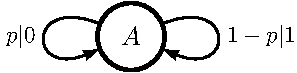
\includegraphics[scale=1.0]{../chapter1/figures/tex/IID}
\end{center}
\caption{IID binary process.}
\label{fig:IID_eM}
\end{figure}

The labeled transition matrices are one-dimensional,
\begin{align*}
T_{A,A}^0 = \begin{bmatrix}p\\\end{bmatrix}, T_{A,A}^1 = \begin{bmatrix}1-p\end{bmatrix}
\end{align*}
This is a rather trivial, but important process to keep in mind because many kinds of data are taken without consideration for temporal correlation. We will see in how many \emph{independent} ways this process class actually is trivial. Let us use this to motivate our discussion of measures of processes.

\subsection{Entropy and Entropy Rate}
The first aspect of a process we would like to characterize is its variability; more precisely, we would like to know the degree of uncertainty in particular groups of random variables. Following Shannon \FIX{cite shannon}, we characterize the uncertainty by the Shannon information.
\begin{Def}
The \emph{Shannon information}, or here the \emph{entropy \footnote{As in most information theory, computer science and symbolic dynamics, the $\log$ function in this work will always mean base two.}}, of a random variable is given by,
\begin{align*}
H[X] &= -\sum_{x \in X}{\Prob(X=x) \log{\Prob(X=x)}}
\end{align*}
Analogously, the entropy of a set of random variables, or their joint probability distribution, is defined, 
\begin{align*}
H[X, Y] &= -\sum_{x \in X, y \in Y}{\Prob(X=x, Y=y) \log{\Prob(X=x, Y=y)}}
\end{align*}
\end{Def}
In the trivial case of our first example (Fig.~\ref{fig:IID_eM}), the uncertainty in the bi-infinite string of random variables is infinite. Each random variable has some finite uncertainty associated with it, and by definition of being IID, the uncertainty in any given variable is independent of any other variable. Therefore, the uncertainty in the entire string is infinite. Since a categorically infinite entropy leaves little to discuss \footnote{Actually there is much to discuss. For continuous time or continous valued output, measures such as the differential entropy will generically be infinite. We hope that a talented mathematician will generalize the ideas here to the continuous case.}, we will be primarily interested in the functional relation between entropy and length scale as the length grows. Furthermore, we are interested in not only the asymptotic behavior (some kind of exponential envelope), but also the finite length behavior. In fact we are more interested in the finite length behavior as long as we are guaranteed \emph{some} kind of convergence. The parent entropy function that many important process features derive from is the block entropy.
\begin{Def}
The \emph{block entropy function} (or curve \footnote{This is a discrete function and so we use the word curve to be suggestive of the fact that these functions are highly restricted by monotonicity and such and so are, as far as discrete functions go, relatively curve-like.}) is is the entropy of the distribution of words at length $L$.
\begin{align*}
H[\MeasSymbol_0^L] = -\sum_{\meassymbol_0^L \in \mathcal{A}^L}\Prob(\MeasSymbol_0^L=\meassymbol_0^L) \log {\Prob(\MeasSymbol_0^L=\meassymbol_0^L)}
\end{align*}
\end{Def}
\FIX{properties: nondecreasing, concave}
\begin{Def}
The \emph{entropy rate}, $\hmu$, of a process is the limit of the conditional entropy,
\begin{align*}
\hmu = \lim_{L \to \infty}{H[\MeasSymbol_0 | \MeasSymbol_{-L}, \MeasSymbol_{-L+1}, \ldots, \MeasSymbol_{-1}]}
\end{align*}
In our shorthand, $\hmu = H[\MeasSymbol_0 | \Past]$.
We are also interested in finite length approximations to the entropy rate,
\begin{align*}
\hmu(L) &= H[\MeasSymbol_0 | \MeasSymbol_{-L}, \MeasSymbol_{-L+1}, \ldots, \MeasSymbol_{-1}]\\
&= H[\MeasSymbol_{-L}, \MeasSymbol_{-L+1}, \ldots, \MeasSymbol_{-1}, \MeasSymbol_{0}] - H[\MeasSymbol_{-L}, \MeasSymbol_{-L+1}, \ldots, \MeasSymbol_{-1}]
\end{align*}
\end{Def}
\FIX{properties: nonincreasing, convex}
The entropy rate estimate at $L=0$ is defined to be $\hmu(0)=\log(|\mathcal{A}|)$. This is just stating that if you know nothing about the process other than the size of the alphabet, your uncertainty is maximal,that is, the entropy of a uniform distribution over the alphabet.
\begin{align*}
H[\frac{1}{|\mathcal{A}|} \times (1,1,\ldots,1)] &= -\sum_{i=1}^N{\frac{1}{|\mathcal{A}|} \log{\frac{1}{|\mathcal{A}|}}}\\
&=\log{|\mathcal{A}|}
\end{align*}
If we think of this geometrically, the entropy rate is the limit of the discrete slope of the block entropy function. Simple geometric features of these key functions will play a primary role in both motivating classifications of processes and also in understanding features otherwise defined.
\begin{figure}[h!]
\centering
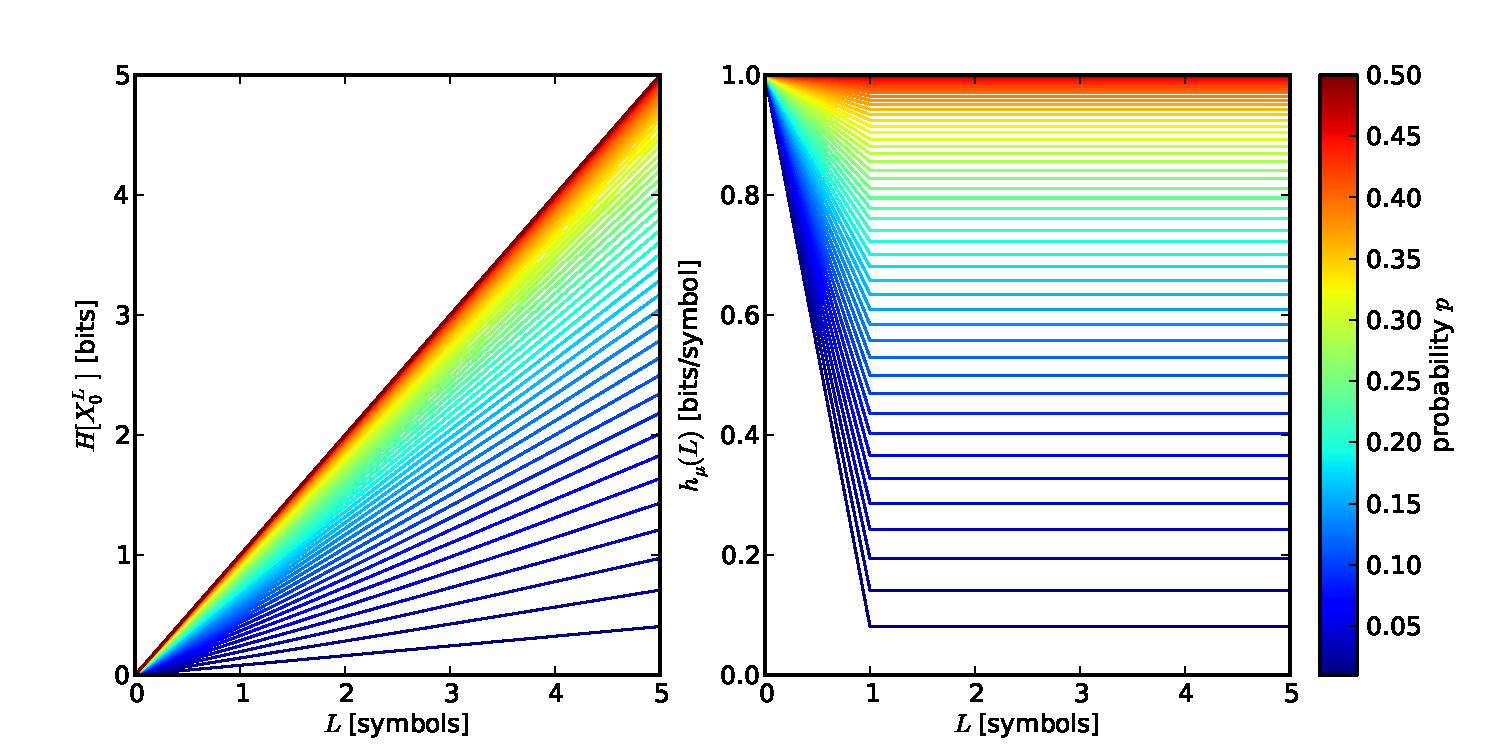
\includegraphics[scale = 0.6]{../chapter1/figures/scripts/BE_IID_all}
\caption{(Left) Block entropy curve for all binary IID processes ($\Prob(\MeasSymbol=0) = p$). Each is simply a line through the origin with slope determined by $p$. Since there is a symmetry in the class about $p=0.5$, only on half of the $p$ values are illustrated. (Right) Finite length entropy rate approximations. Colorbar indicates the probability, $p$, that is varied to obtain different members of a process family. The particular probability, $p$, refers to the variable in Fig.~\ref{fig:IID_eM}.}
\label{fig:BE_IID_all}
\end{figure}
We can write the probability distribution for an IID process as a product of distributions for each random variable.
\begin{align*}
\Prob(\Past, \Future) = \ldots \times \Prob(\MeasSymbol_{-1}) \times \Prob(\MeasSymbol_{0}) \times \Prob(\MeasSymbol_{1}) \ldots
\end{align*}
As a consequence, the block entropy is linear in the length, $L$.
\begin{align*}
H[\MeasSymbol_0^L] &= -\sum_{\meassymbol_0^L \in \mathcal{A}^L}\Prob(\MeasSymbol_0^L=\meassymbol_0^L) \log {\Prob(\MeasSymbol_0^L=\meassymbol_0^L)}\\
&= -\sum_{\meassymbol_0, \meassymbol_1,\ldots,\meassymbol_{L-1} \in \mathcal{A}}\Prob(\MeasSymbol_0=\meassymbol_0) \times \ldots \times \Prob(\MeasSymbol_{L-1}=\meassymbol_{L-1}) \log {\Prob(\MeasSymbol_0=\meassymbol_0) \times \ldots \times \Prob(\MeasSymbol_{L-1}=\meassymbol_{L-1})}\\
&= -\sum_{x_0 \in \mathcal{A}}{\Prob(\MeasSymbol_0 = \meassymbol_0 \log{\Prob(\MeasSymbol_0 = \meassymbol_0)})} - \ldots 
-\sum_{x_{L-1} \in \mathcal{A}}{\Prob(\MeasSymbol_{L-1} = \meassymbol_{L-1} \log{\Prob(\MeasSymbol_{L-1} = \meassymbol_{L-1})})}\\
&= - L \times \sum_{x_0 \in \mathcal{A}}{\Prob(\MeasSymbol_0 = \meassymbol_0) \log{\Prob(\MeasSymbol_0 = \meassymbol_0)}}\\
&=-L H[\MeasSymbol_0]
\end{align*}
An immediate consequence of this is that the entropy rate is equal to the length-one approximation.
\begin{align*}
\hmu &= \lim_{L \to \infty}{H[\MeasSymbol_0^{L}] - H[\MeasSymbol_0^{L-1}]}\\
&= \lim_{L \to \infty}{L H[\MeasSymbol_0] - (L-1)H[\MeasSymbol_0]}\\
&= H[\MeasSymbol_0]
\end{align*}
That is, beyond considering the most trival statistic, there is nothing more to learn about this system. Since this entropy, or entropy rate, will arise rather frequently, it is often referred to simply as the \emph{binary entropy} and denoted $H(p)$.

A more interesting process is one for which the finite length approximations to $\hmu$ are something other than constant. A very simple example that illustrates this \footnote{In fact, \emph{any} process other than IID will illustrate this. I have just chosen a simple one that is convenient because it is simple in other ways.} is the Golden Mean Process (Fig.~\ref{fig:GM_eM}).
\begin{figure}[h!]
\centering
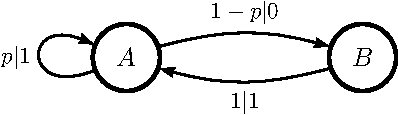
\includegraphics[scale = 1.0]{../chapter1/figures/goldenmean_feM_gr}
\caption{The Golden Mean Process is one that disallows consecutive zeros. After a zero [one] is seen, the process is in causal state $B$ $[A]$.}
\label{fig:GM_eM}
\end{figure}
Notice that in Fig.~\ref{fig:BE_GM_all}, the entropy rate estimates reach the entropy rate at $L=2$. To restate, for the Golden Mean process, the conditional uncertainty in every symbol, including and beyond the second, is $\hmu$. 
\begin{align*}
H[\MeasSymbol_0 | \MeasSymbol_{-k}, \ldots, \MeasSymbol_{-1}] = H[\MeasSymbol_0 | \MeasSymbol_{-1}] = \hmu
\end{align*}
This leads one to naturally speculate that there is a conditional \emph{probabilistic} independence as well as this conditional \emph{entropic} independence. This is true, but because it is an intuitive result with a somewhat inelegant proof, it can be found in App.~\ref{app:proofs}
\begin{figure}[h!]
\centering
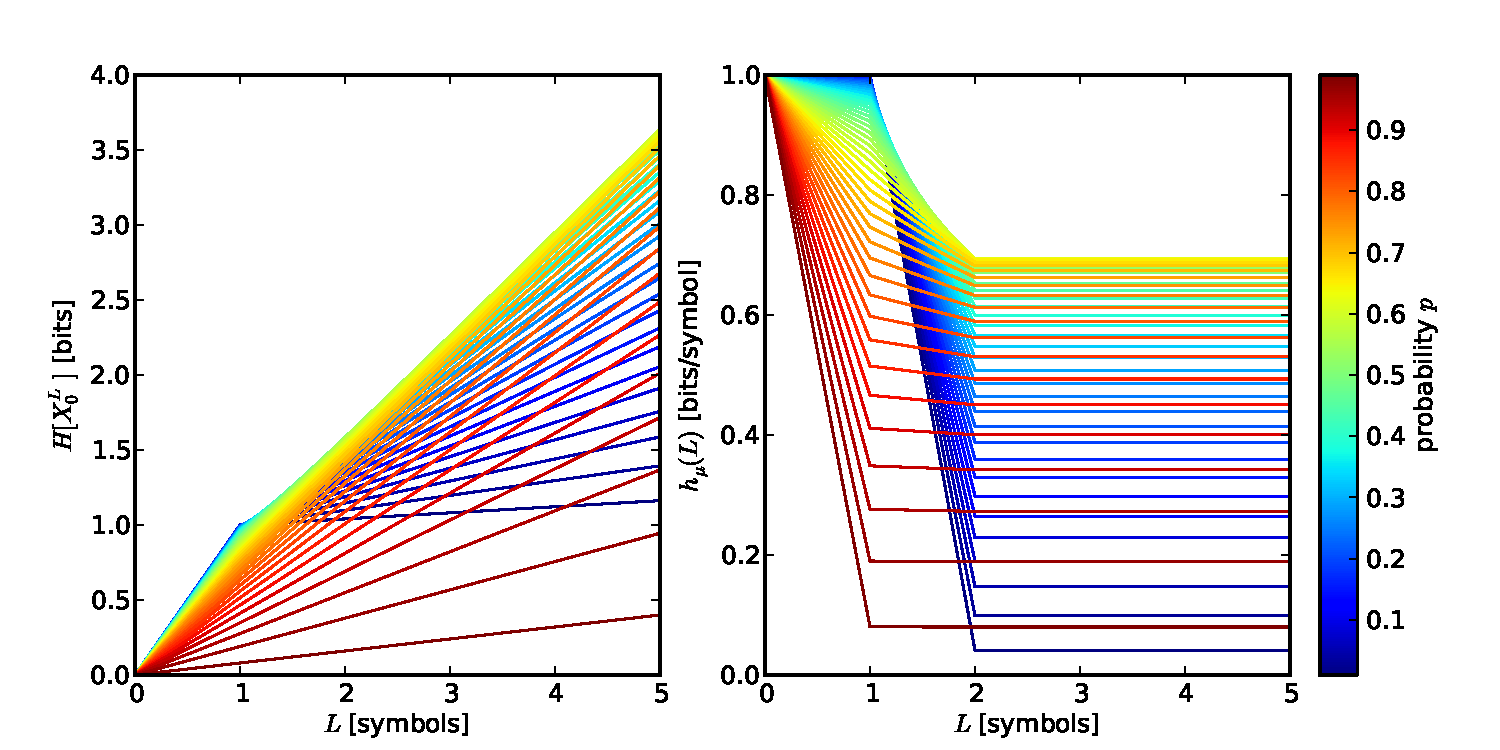
\includegraphics[scale = 0.6]{../chapter1/figures/scripts/BE_GM_all}
\caption{(Left) Block entropy curves for all Golden Mean processes. Each is linear for $L\ge1$. (Right) Each finite length entropy rate estimate reaches its asymptotic value $\hmu$, at $L=2$. This indicates that the additional uncertainty in the $L=2$ blocks, beyond the $L=1$ blocks, is already $\hmu$. This implies that the minimum correlation length required for maximal prediction ability is $L=1$. That is, the Golden Mean is an \order{1} Markov process.}
\label{fig:BE_GM_all}
\end{figure}
We should be sure to point out an important feature of the \eM. In contrast with generic hidden Markov models, the \eM\ has the property that the entropy rate can be calculated directly from it. We argue that this is a consequence of the \eM\ being the natural representation of the process. 

Now that the entropy rate has been defined as a limit and is certainly straightforward enough to estimate, we should look for a closed form. We might imagine that, for any hidden Markov model (composed of states $\AlternateState$), that the time average surprise is the same as the state average surprise (when weighted by state visitation probabilities). Specifically, that
\begin{align*}
\hmu \stackrel{?}{=} \sum_{\alternatestate}{\Prob(\AlternateState_0 = \alternatestate) H[\MeasSymbol_0 | \AlternateState_0 = \alternatestate])}
\end{align*}
It is easy to see that this is not true. Consider a nonunifilar presentation of the Golden Mean Process. The conditional entropies are $H[\MeasSymbol_0 | \AlternateState_0=A] = 0$ and $H[\MeasSymbol_0 | \AlternateState_0=B] = 0$. No weighted sum of these conditional entropies will yield what we know to be a non-zero entropy rate.
\begin{figure}[h!]
\centering
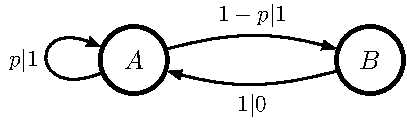
\includegraphics[scale=1.0]{../chapter1/figures/tex/GM_nonunif}
\caption{Nonunifilar presentation of the Golden Mean Process. The entropy rate of the process is \emph{not} simply the weighted average of the entropies of symbols emitted after visiting each state.}
\label{fig:GM_nonunif}
\end{figure}
The correct form for the entropy rate is in fact this weighted sum of individual state entropies, but \emph{only} when the states in question are \emph{causal} states. So for \eMs, we have the following closed form for the entropy rate in terms of causal state asymptotic probabilities and transition probabilities.
\begin{align*}
\hmu & = H[\MeasSymbol_0|\CausalState_0] \\
&=\sum_{\causalstate \in \mathcal{A}}{\Prob(\CausalState_0 = \causalstate) H[\MeasSymbol_0 | \CausalState_0 = \causalstate])}\\
  & = - \sum_{\causalstate \in \CausalStateSet} \Pr(\CausalState)
  \sum_{\meassymbol \in \mathcal{A} \causalstateprime \in \CausalStateSet} T^{(\meassymbol)}_{\CausalState \CausalState^\prime}
  \log_2 \sum_{\causalstateprime \in \CausalStateSet}{T^{(\meassymbol)}_{\CausalState\CausalState^\prime}}
\end{align*}

\section{Statistical Complexity}
Above, $\Pr(\CausalState)$ is the asymptotic probability of the causal states, which is obtained as the normalized principal eigenvector
of the transition matrix $T = \sum_{\{x\}} T^{(x)}$.  We will use $\pi$ 
to denote the distribution over the causal states as a row vector.\footnote{The matrix algebra here follows the `state on the left, transition matrix on the right' convention.} 
This distribution over states leads to a second fundamental characterization of processes---the statistical complexity.
\begin{Def}
A process's \emph{statistical complexity}, $\Cmu$, can be directly calculated
from its \eM\ as it is a property of the dynamic over the causal states:
\begin{align}
\Cmu
   & = H[\CausalState] \nonumber \\
   & = - \sum_{\{\CausalState\}} \Pr(\CausalState) \log_2 \Pr(\CausalState) ~.
\end{align}
\end{Def}
The statistical complexity is a \emph{statistical} complexity as opposed to a deterministic one, such as Kolmogorov complexity,\footnote{Kolmogorov complexity is also known as: descriptive complexity, Kolmogorov-Chaitin complexity, stochastic complexity, algorithmic complexity, algorithmic entropy, and program-size complexity.} meaning that the measure is intended to capture the complexity of a class of data rather than a particular instance. To illustrate, a coin may be flipped to generate a variety of sequences. One such sequence is an alternating sequence of heads and tails, $(HT)^N$. This sequence may be generated by the compact\footnote{We call this compact because as the size of the program goes as $\log(N) + C$. Thus the limit of the ratio of output sequence size to program size is zero. This indicates that this subprocess has and entropy rate of zero.} program: i=0,for(i<N)\{write H, write T, i=i+1\}. The increasing majority of sequences will not have this compactness, yet all are possible realizations of the output of this simple dynamical system. The goal of a statistical complexity is to provide a characterization of all of these possiblilities.

Why should we aim to describe the broad class behavior rather than the detailed behavior indicated by a particular data string? If our aim is to describe the physical dynamical system, and if we believe that this system has inherent unpredictability, then describing a particular instance, as the Kolmogorov complexity would do, might actually \emph{overspecify} the physical system. For instance, a flipped coin could certainly produce a binary representation of $\pi$; another might code for the name of the next president. Neither one of these things captures the essence of the physical system---that it is IID and uniformly\footnote{Some might argue that we have to toss the coin with more vigor (see \FIX{diaconis coin}).} random heads and tails. If we insist on characterizing the coin's behavior by the two instances above, then I argue that we ought to consider \emph{all} possible instances. This is clearly not a productive use of time.

What exactly is the statistical complexity telling us? As $\Cmu$ is defined as the entropy of a probability distribution over some event space, it can immediately be understood in the context of communication theory. If Alice wishes Bob to synchronize his ensemble of identical dynamical systems to hers, she must communicate $\Cmu$ bits per member of the ensemble.\footnote{Of course she must communicate $\Cmu$ bits \emph{on average}, but that is the standard assumption made in information theory. In fact, without it, information does not have the same meaning.} If it is $\Cmu$ bits that is passed to Bob to describe the state of the system, then it could be said that each system \emph{carries} that amount of information. This is why the statistical complexity is interpreted as \emph{stored information}.

Why is this a good measure of complexity? As we live in a world where complexity measure abound, it is important to pause and reflect on the particular contribution of a particular measure. We first claim that the above description of $\Cmu$ as stored information is strong evidence for its naturalness. Additionally, it has some properties that although somewhat trivial, are not shared by all. In thinking about the range of possible processes, it is hard to argue that IID processes are not on \emph{some} particular extreme. Correspondingly, the statistical complexity of any IID process is zero. This seems to satisfy our intuition about what a complexity measure ought to say about IID processes. In another corner of process space lie completely predictable. These processes, certainly for finite cases, are just the periodic ones. The statistical complexity of these will be the log of the period length. Another good reason is that $\Cmu$ has a kind of extensivity. If two uncorrelated processes are `placed side-by-side', which is the usual thing to do when testing for extensivity, the joint process characterized by the process language over the appropriate tuples of symbols has a statistical complexity which is simply the sum of the individual complexities.\footnote{I might argue that this way of thinking about extensivity is a little mundane. The side-by-side test for extensivity is born of thinking about equilibrium systems. As \eMs\ are definitely not equilibrium systems, it would be most interesting to test for extensivity in different ways. One might sample from the two systems in an alternating manner. We can imagine something more drastic, and maybe harder to motivate, like the graph-join of the two \eMs. Presently, only little is known about about the consequences of these types of actions.}

Thus, the \eM\  directly gives two important properties: a process's rate
($\hmu$) of producing information and the amount ($\Cmu$) of historical
information it stores in doing so.

\section{Excess Entropy}

The entropy rate is a property that comes straight out of communication theory. In that context, it is the minimum capacity of an error-free channel; equivalantly, it is the amount of supplementary information required for maintaining perfect decoding (which we think of as prediction). Another concept that arises very naturally in the communication context is the transference of information from input to ouput. Different channels, depending on their capacity, noise present, etc., will have varying abilities to transfer information from one side of the channel to the other. We can cast a dynamical system or time-series as a channel in the following way; The past is considered the input, the future is the output, and the channel itself is the \eM. Given this picture, the excess entropy is the amount of information about the past that is transmitted via the \eM\ channel to the future (See Fig.~\ref{fig:CommunicationChannel}). We express this mathematically in terms of a mutual information.
\begin{align*}
I[\Past ; \Future] = \EE
\end{align*}
Excess entropy has gone by several different names and has been reinvented several times \FIX{cite early JPC, Grassberger, etc}. There are several equivalent forms for $\EE$, see Ref.~\cite[and references therein]{Crut01a}. Here we quote the definition of excess entropy from Ref.~\FIX{RURO}, where the name is somewhat more intuitive.
\begin{Def}
The \emph{excess entropy} is the sum over word lengths of the degree to which the entropy rate estimate is in excess of the true entropy rate.
\begin{align*}
\EE = \lim_{L' \to \infty }{\sum_{L=1}^{L'}{(\hmu(L) - \hmu})}
\end{align*}
\end{Def}
Excess entropy, and related mutual information quantities, are widely used
diagnostics for complex systems. They have been applied to detect the
presence of organization in dynamical systems~%
\cite{Fras90b,Casd91a,Spro03a,Kant06a}, in spin systems~%
\cite{Arno96,Crut97a,Feld98b}, in neurobiological systems~%
\cite{Tono94a,Bial00a},
and even in language, to mention only a few applications. For example, in
natural language the excess entropy ($\EE$) diverges with the number of
characters $L$ as $\EE \propto L^{1/2}$. The claim is that this reflects the
long-range and strongly non-ergodic organization necessary for human
communication~\cite{Ebel94c,Debo08a}.

It can be demonstrated that this definition is, at least for the types of processes studied in this thesis,\footnote{Extensions as benign as the addition of an extra dimension---to a 2D process---necessitate more care with these equivalences \FIX{cite feldman 2D}.} equivalent to the mutual information concept.
\begin{align*}
I[\Past;\Future] &= \lim_{L \to \infty}{I[\MeasSymbol_{-L}^{L};\MeasSymbol_0^{L}]}\\
&= \lim_{L \to \infty}{H[\MeasSymbol_{-L}^L] + H[\MeasSymbol_0^{L}]-H[\MeasSymbol_{-L}^{L}, \MeasSymbol_0^{L}]}\\
&= \lim_{L \to \infty}{H[\MeasSymbol_{0}^L] + H[\MeasSymbol_0^{L}]-H[\MeasSymbol_0^{2L}]}\\
&= \lim_{L \to \infty}{2H[\MeasSymbol_{0}^L] -H[\MeasSymbol_0^{2L}]}\\
&= \lim_{L \to \infty}{2(H[\MeasSymbol_{0}^L] - L\hmu) -H[\MeasSymbol_0^{2L}] + 2L\hmu}\\
&= \lim_{L \to \infty}{2\sum_{L'=1}^{L}{(H[\MeasSymbol_{0}^{L'}] - H[\MeasSymbol_0^{L'-1}] - \hmu)} -\sum_{L'=1}^{2L}{(H[\MeasSymbol_0^{L'}] -H[\MeasSymbol_0^{L'-1}] + \hmu)}}\\
&= \lim_{L \to \infty}{2\sum_{L'=1}^{L}{(\hmu(L') - \hmu)} -\sum_{L'=1}^{2L}{(\hmu(L') + \hmu)}}\\
&= 2\lim_{L \to \infty}{\sum_{L'=1}^{L}{(\hmu(L') - \hmu)}} -\lim_{L \to \infty}{\sum_{L'=1}^{2L}{(\hmu(L') + \hmu)}}\\
&= 2 \EE - \EE = \EE
\end{align*}
The second line follows from the definition of mutual information. The third line is a result of stationarity. We insert some copies of $\hmu$ and rearrange to form the definition of \EE. To split the limit into two, we assume the existence of the individual limits. This really amounts to assuming the existence of one limit---\EE. In recent work, see Ref.~\FIX{nick}, it is shown that this limit exists for all \eMs\ with a finite number of states.
\begin{figure}[h!]
\centering
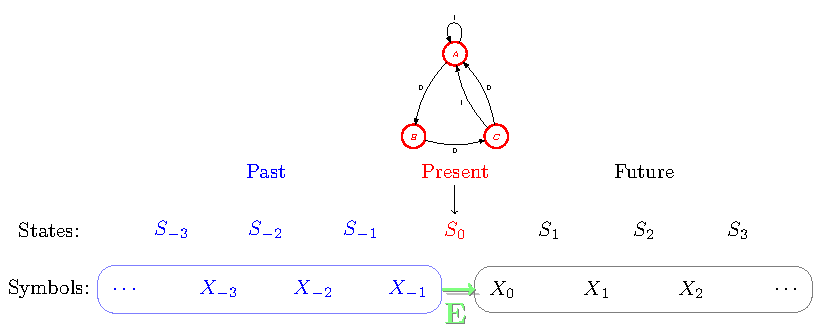
\includegraphics[scale=1.1]{../chapter1/figures/tikz/CommunicationChannel}
\caption{A stochastic process can be viewed as a communication channel. The data in the past is the input to the channel. The channel itself is the dynamical system, or \eM, which transmits information to the future. The total information transmitted from past to future is equal to the excess entropy.}
\label{fig:CommunicationChannel}
\end{figure}

We can begin to collect our understanding of the information theoretic relationships among \eM\ variables using an I-diagram (see Fig.~\ref{fig:2var_IXYisE}). For a review of I-diagrams, see App.~\ref{app:Venn}. The other two quantities shown in this diagram are $H[\Past | \Future]$ and $H[\Future | \Past]$. Since these will generally be infinite quantities, it can be useful to think of the random variables in their finite forms, $\MeasSymbol_{-k}^k$ and $\MeasSymbol_0^k$. The rate of growth of these agglomerated variables (with $L$) is bounded above by $H[\MeasSymbol_0]$ and below by $\hmu$.
\begin{figure}[h!]
\centering
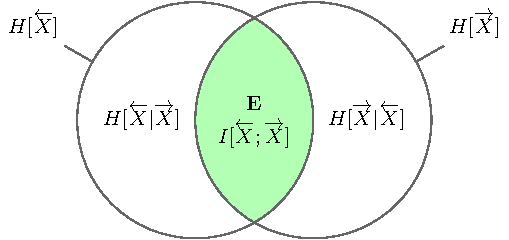
\includegraphics{../chapter1/figures/tikz/2var_IXYisE}
\caption{This I-diagram highlights the role of excess entropy as the mutual information between past and future data.}
\label{fig:2var_IXYisE}
\end{figure}

To form a complete I-diagram for an \eM, we must introduce a state variable. Of course this diagram is not a complete description, but it does aid our thinking in several ways. We start by adding a generic state, actually any random variable at all will do. In Fig.~\ref{fig:3var_PastFutureRcolored}, all possible information relations among the variables are listed.
\begin{figure}[h!]
\centering
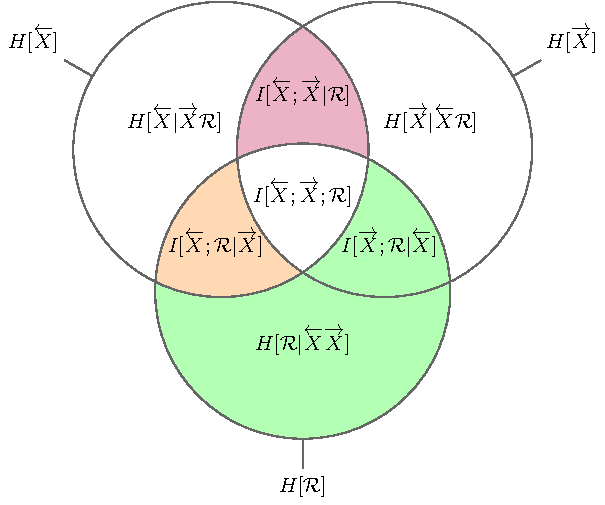
\includegraphics{../chapter1/figures/tikz/3var_PastFutureRcolored}
\caption{The generic relation among the past, future and a state, $\AlternateState$ includes 15 nontrivial information quantities. Demanding that the state involved is a causal state effects 4 of these quantities. The green area (which corresponds to two information atoms) is zero because the causal state is a single-valued function of the past. The purple area is zero because causal states are prescient. The orange area is not zero, but is the minimum value possible, given that green and purple are zero.}
\label{fig:3var_PastFutureRcolored}
\end{figure}

Note that some of the region are colored. This is to indicate that there is a difference between a generic state variable and a \emph{causal} state in so far as these areas \footnote{The words `area', `region', `[information] quantity' and `[information] atom' are used interchangeably here in light of the correspondence between Venn diagrams and information theory. For more about this relationship refer to App.~\ref{app:Venn}.} are concerned. Let us explore these individually, substituting a causal state, $\CausalState$ for the generic state, $\AlternateState$.

The green area is zero because the causal state is a single-valued function of the infinite past, $\past$. Since $H[\CausalState|\Past \Future]$ is also a conditional entropy, and therefore positive, we have that the green subregions are individually zero.

The purple region is zero because the probability distribution over futures given a past is the same as that given the induced causal state. This implies that a past and the causal state it induces share the same amount of information with the future. Since we already have that $I[\Future ; \CausalState | \Past] = 0$, this shared information must be the \emph{same} information. Recalling that $I[\Past ; \Future] = \EE$, we then arrive at $I[\CausalState ; \Future] = \EE$.

The orange region is generically not zero, although the \eM\ ensures that it is, given that the previously describe regions are zero, the smallest possible value. It is this orange region that will be the subject of much discussion later on. It is a quantity governed by opposing forces; on the one hand, it must be large enough to accomodate capturing all of the information relevant to the future (\EE), while on the other hand it is asked to be as small as possible, giving the minimal unifilar optimally predictive representation. This quantity is called the crypticity.

\section{Estimation of Excess Entropy}

The difficulty in obtaining accurate estimates of the excess entropy in even relatively benign systems was the primary (initial) impetus behind our effort to reframe this problem. This section is not intended to provide a comprehensive accounting of the various ways in which estimation can be difficult, nor will it quantify exactly how difficult the estimation is. We will see through a simple example that it is indeed difficult, and argue that this is generic enough to warrant searching for an alternate method. The method having been discovered and detailed in Ref.~\FIX{PRATISP} obviates the need to revisit and detail the previous study of difficulty in estimation. \FIX{a little boring}

\subsection{Example of Sharp Convergence : Order-3 Markov}

In order to set the stage for the difficult estimation task in the next section, we interrupt to offer an apparently substantial process to contend with (see Fig.~\ref{fig:random_order3}). This process, being an order-3 Markov process, is a fair test case for estimation algorithms as finite order Markov models are used in a wide variety of settings \FIX{cite some Markov modeling refs}.

\begin{figure}[h!]
\centering
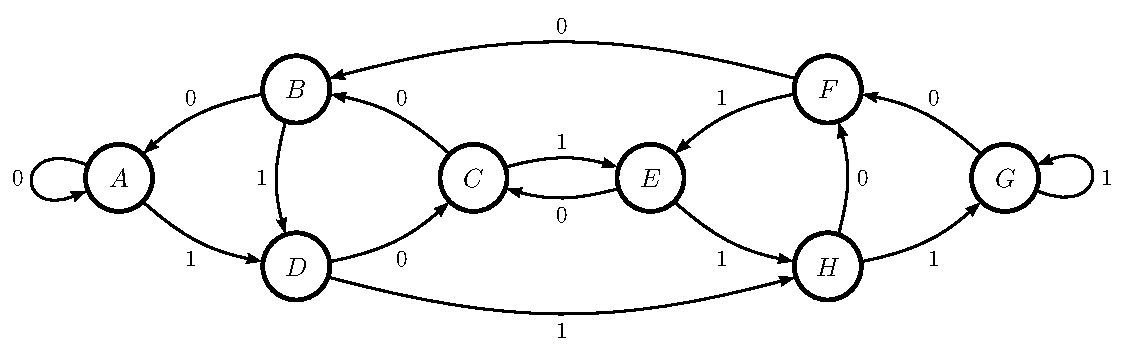
\includegraphics[scale = 0.6]{../chapter1/figures/tex/mc3_tr}
\caption{A process with 8 causal states. Since each state has two outgoing transitions, each of which has one free parameter, we suppress the probabilities here. The reader may verify that this is the structure of an order-3 Markov process---any 3 symbols will uniquely define a state (the converse happens to also be true in this instance).}
\label{fig:random_order3}
\end{figure}

Calculating the standard excess entropy estimates, we see in Fig.~\ref{fig:E_random_order3} that for all instances of the class, there is a sharp convergence at $L=3$. This is a consequence, and additionally an indicator, of the process being order-3 Markov. In fact, excess entropy can be calculated for finite order Markov processes in a finite way. Since we have that the entropy rate estimate becomes exact at $L=R+1$ for an order-R markov process. This has the effect of truncating the infinite sum,
\begin{align*}
\EE &= \sum_{L=1}^{\infty}(\hmu(L) - \hmu)\\
&= \sum_{L=1}^{R}(\hmu(L) - \hmu)\\
&= H[\MeasSymbol_0^R] - R \hmu.
\end{align*}

The last step is accomplished by collapsing the telescoping sum of entropy rate estimates. It appears that for finite order Markov processes, certainly for small orders, the excess entropy is easily calculable. We should now ask the questions: ``What happens as the Markov order becomes large?'', and ``What happens when the process is not finite order Markov?''

To answer the first question, we have to calculate the probabilities of roughly $|\mathcal{A}|^R$ different length-$R$ words. The number of words will be smaller than this depending on the process's forbidden words. For large alphabets and large orders, this can quickly become a challenging task. For instance, if we treat the English language as a Markov process over letters $\{a, \ldots, z\}$and allow for a very modest correlation length of 6, we find that there is not even enough space on a modern computer to store the resulting probability distribution.

\begin{figure}[h!]
\centering
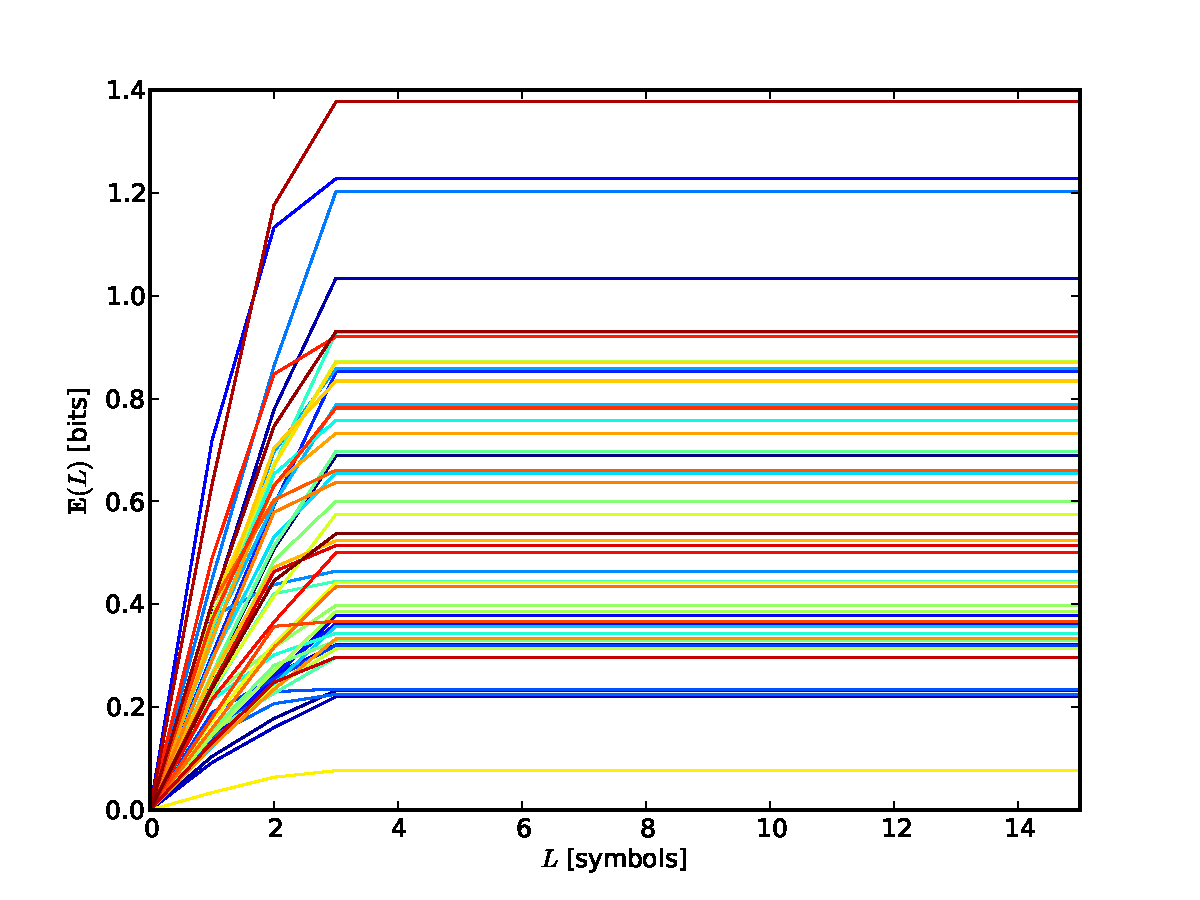
\includegraphics[scale = 0.45]{../chapter1/figures/scripts/E_random_order3}
\caption{Excess entropy estimates for 50 instances of full order-3 Markov chains (see Fig.~\ref{fig:random_order3} for the topology). Notice that the estimates become extremely good (actually exact) at $L=3$. This is a consequence of the process being finite order Markov.}
\label{fig:E_random_order3}
\end{figure}

To illustrate the reponse to the second question, let us investigate a very simple non-Markov process.

\subsection{Example of Slow Convergence : Even Process}
The example we use to illustrate this complication is the Even Process, as seen in Fig.~\ref{fig:even_feM_gr}. The reason that this process is an appropriate choice for illustrating difficulty with convergence is that it is not Markovian; we might say that it is infinite-order Markov. This can be intuitively understood in the following way: If we have access to only a finite symbol history, say $N$ symbols, then when we encounter a word of $N$ ones, we cannot provide the proper distribution over futures. At a coarse level, we don't know whether the sequence is currently even in length and therefore has the option of terminating with a zero, or if it is currently odd in length and therefore \emph{must} continue with at least one more one. Therefore no finite history (finite order Markov) model can properly generate the Even Process. This is a fundamental difference\footnote{This fundamental difference is \emph{not} the difference between node output models and edge output models. Given a unifilar edge output model (this is a `hidden model') with $N$ nodes and $M$ symbols, there are at most $N \times M$ edges. The corresponding node output model (also a `hidden' model) then trivially has at most $N \times M$ nodes. This difference is of course important, but never involves transforming a 2 state model to an infinite state model} between Markov models, or chains; and hidden Markov models, or functions of Markov chains \FIX{cite Markov vs hidden Markov}.
\begin{figure}[h!]
\centering
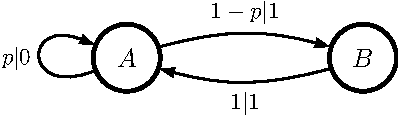
\includegraphics[scale = 1.0]{../chapter1/figures/even_feM_gr}
\caption{The Even Process requires that all blocks of uninterrupted ones, with zeros on either side, be even in length.}
\label{fig:even_feM_gr}
\end{figure}

\begin{table}
\centering
\begin{tabular}{|c|c|c|}
\hline
 Prediction & $N$ even & $N$ odd \\ \hline
$\Prob(\MeasSymbol_N = 0 | \MeasSymbol_0 = 1, \ldots, \MeasSymbol_{N-1}=1)$ & $1-\frac{p}{2}$ & $\frac{p}{2}$\\
$\Prob(\MeasSymbol_N = 0 | \MeasSymbol_{-1} = 0, \MeasSymbol_0 = 1, \ldots, \MeasSymbol_{N-1}=1)$ & $p$ & 0 \\
$\Prob(\MeasSymbol_N=0 | \CausalState_N=A)$ & $p$ & --\\
$\Prob(\MeasSymbol_N=0 | \CausalState_N=B)$ & -- & 0 \\
\hline
\end{tabular}
\caption{The above table illustrates that for the Even Process, for any length $N$, there exists a word (all ones) such that prediction based on that word alone is different than prediction based on that word knowing that the previous symbol is 0. Notice that the optimal probabilities, those predicted after the block of ones is begun by a zero, are the same as those predicted by the appropriate induced causal state.}
\label{tab:EvenProcessProbs}
\end{table}

It is plain to see in the left pane of Fig.~\ref{fig:E_hmu_Even_all_reldiff} that, for a substantial subset of instances, the relative errors in the excess entropy estimates do not fall within acceptable bounds even when considering correlation lengths up to 10. The excess entropy, defined as the infinite sum of the entropy rate overestimates, is continually being fed by new overestimates, as is seen in the right pane of Fig.~\ref{fig:E_hmu_Even_all_reldiff}. One should probably object at this point saying that with appropriate algorithms and compute power, lengths far beyond 10 must certainly be accessible. This objection is certainly valid, but misses the point of the illustration. First, this is only the `simplest of the difficult' examples. Depending on the application, model sizes will have dozens or hundreds of nodes. Second, as a matter of theoretical investigation, we would like to be able to calculate the excess entropy for infinite \eMs. Any previous algorithm will fail in this task. Third, the brute force griding out of ever better approximations does not strike us as the proper way to really understand how excess entropy behaves. To illustrate, reverse-type questions about $\EE$ are difficult to resolve numerically: The question, ``for what value of $p$ does $\EE=1/\pi$?'' poses a reasonable computational challenge. Presumably one would have to sample points in the range of $p$, estimate \EE\ for each, and through interpolation and possibly some manner of successive approximation, hone in on the correct value. This is of course possible, but completely non-generalizable. To examine some other \EE\ value might require resampling a different region of $p$ values. Furthermore, the addition of a single state would require starting the whole procedure from scratch.

\begin{figure}[h!]
\centering
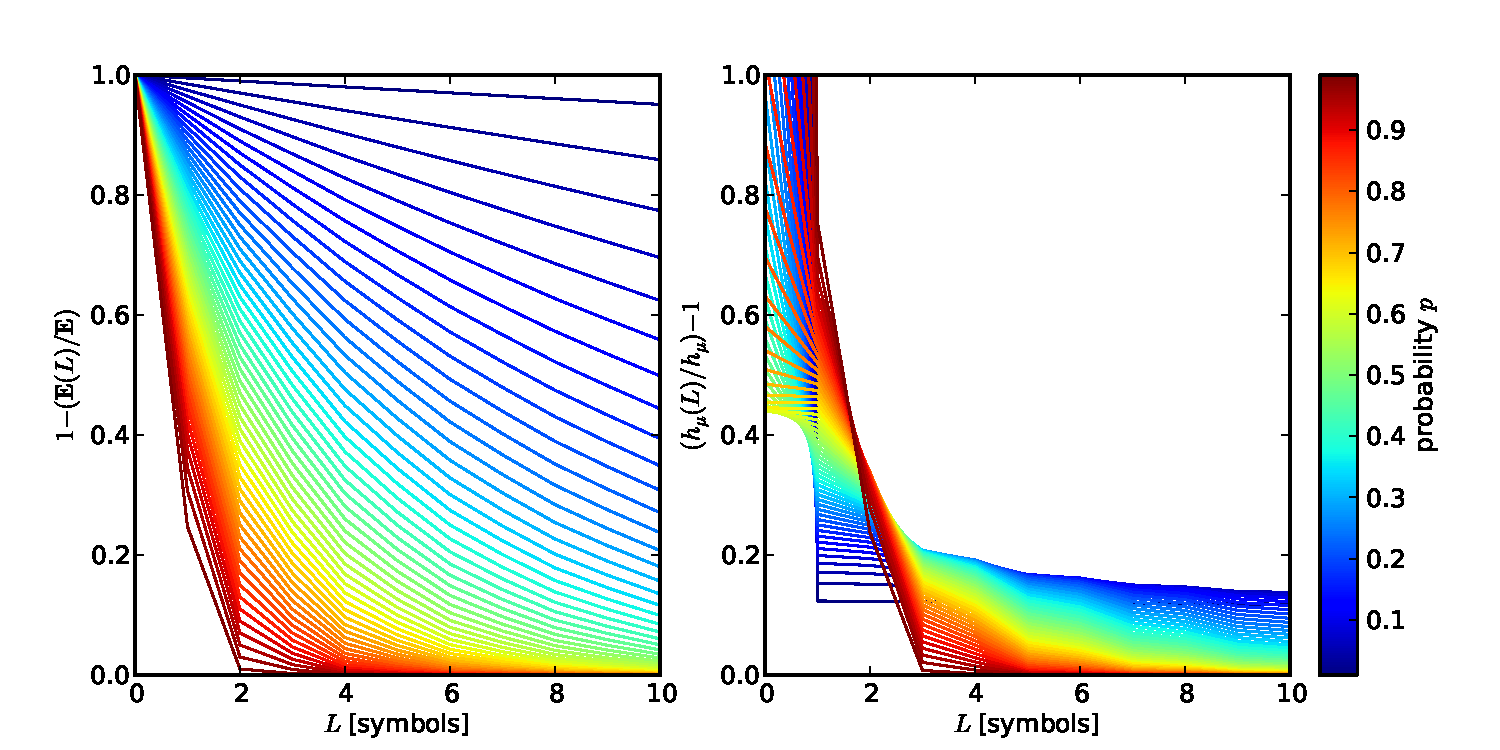
\includegraphics[scale = 0.6]{../chapter1/figures/scripts/E_hmu_Even_all_reldiff}
\caption{The non-Markovianness of the Even Process leads to some members of the family having very slow convergence. (Left) Relative errors in the excess entropy estimates show that even considering correlation lengths up to 10 is grossly inadequate for a large collection of processes. (Right) Relative error of entropy rate estimates are very slow to approach zero for members on the blue end of the spectrum. This process serves as a key motivating example in the search for analytic forms for \EE.}
\label{fig:E_hmu_Even_all_reldiff}
\end{figure}

We would also like to note that the ability to even represent the relative error in the excess entropy estimates, as in Fig.~\ref{fig:E_hmu_Even_all_reldiff}, is only made possible by making use of the algorithm we developed to determine the exact value of \EE. Before access to the limit that our estimates were allegedly approaching, excess entropy estimate plots were much more undetermined. Figure~\ref{fig:E_Even_all} demonstrates the slow, indeterminate growth of the estimates. There is of course the bound from \FIX{shalizi} $\EE \le \Cmu$, but from this simulation, there is no clear way to bound any instance away from $\Cmu$ at all.
\begin{figure}[h!]
\centering
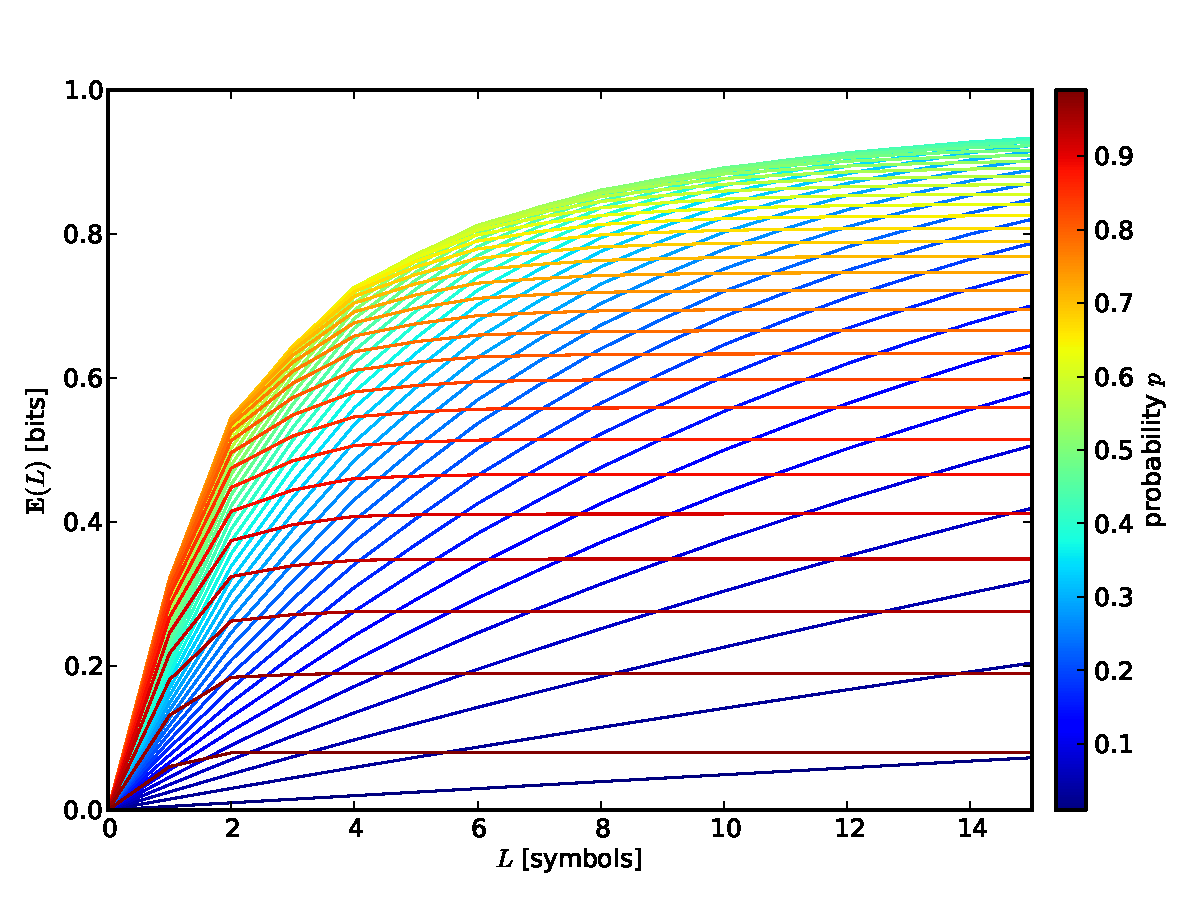
\includegraphics[scale = 0.45]{../chapter1/figures/scripts/E_Even_all}
\caption{Excess entropy estimates for the Even Process without access to the actual limit \EE. Its estimates increase in a very slow manner making claims about convergence, except for very trivial ones, difficult.}
\label{fig:E_Even_all}
\end{figure}

In Ch.~\ref{PRATISP} we present our method for calculating \EE\ for an entire parameterized family of \eMs\ at once. Moreover, this method is finitely terminating even for infinite order Markov processes \footnote{There are some questions remaining as to what happens in the case of infinite transient states. It appears that when the recurrent states are reachable, that this algorithm will be finite despite the infinite transients. The algorithm needs only to reach all recurrent states (not to reach them via all possible transient paths). When the recurrent states are not reachable, it is known that in some cases, one can define an infinite sequence that converges to the correct result and find the limit analytically. It is hoped that this procedure can be made general. As transient states and infinite states are not discussed here, the reader should look for results in the upcoming Ref.~ \FIX{cite Extension of E algo to infinite}}. To put some concreteness to the technique, it can be rapidly calculated by hand that the solution to the above challenge is the result of this equation,
\begin{align*}
\frac{1}{\pi} = \log(2-p) - \frac{1-p}{2-p} \log(1-p).
\end{align*}

\section{Crypticity and Cryptic Order}
The study of the structure of stochastic processes through their \eM\ representations has lead to the the recognition of two new and important quantities: the crypticity, and the cryptic order. Intuitively, these two ideas spring from focusing one's attention not on the information region associated most directly with prediction---the excess entropy or predictive information---but rather with the region that characterizes the information above and beyond $\EE$ necessary for determining the causal state, and thereby for making predictions. This is what we call the crypticity.

\subsection{Crypticity}
\begin{Def}
The \emph{crypticity} , $\PC$, of a process is defined,
\begin{align*}
\PC = H[\CausalState_0 | \Future_0]
\end{align*}
\end{Def}

We represent this quantity in our I-diagram as the difference between the statistical complexity and the excess entropy (see Fig.~\ref{fig:3var_PastFutureS}). At first, it might seem as though the definition of the \eM\ ought to obviate any information except for that which is predictive information. The \eM\ is, after all, the causal representation of the process. How can we reconcile these intuitions? The essential idea is this: optimal prediction, which is what causal states are built for, requires not only the ability to match up histories with the appropriate future, or set of futures; it also requires the ability to match up histories with the appropriate distribution over futures, and \emph{these pairings can overlap}.

A positive crypticity means that despite all your hard work in noting the relations between pasts and futures, and determining which class of pasts you are in, there exists a particular future which can follow more than one class (even all classes) of pasts. Supposing that future is realized, you might wish you had been less careful, as the result might\footnote{There's the rub.} have been the same. To say this a little differently, and mathematically,
\begin{align*}
\underbrace{H[\MeasSymbol_0^L] - H[\MeasSymbol_0^L | \CausalState_0]}_{\text{net earnings}} = \underbrace{H[\CausalState_0]}_{\text{gross earnings}} - \underbrace{H[\CausalState_0 | \MeasSymbol_0^L]}_{\text{taxes}}.
\end{align*}

To expand upon this interpretation a little, the `gross earnings' is the amount that enters consideration. The `net earnings' is the amount of useful resource. Trivially the, the difference is what is given up in `taxes'. This analogy is appealing and correct in that only in very rare cases can you get away with paying no taxes \footnote{It is not claimed that this is a deep analogy, but the `economics of information' is an attractive thought; it suggests competition and optimization. It also encourages us to search for off-shore [quantum] information accounts. Other analogies have been explored for the crypticity, most notably in the context of heat engines. There, the statistical complexity is likened to heat transference and excess entropy to the derived work. The ratio then is a measure of the `thermodynamic efficiency of the machine. There is much work yet to be done to firmly establish an economic or thermodynamic relationship.}.

It is the last term---taxes---which is our crypticity. To assure the reader that this information waste is not just a corner-case, note that the Golden Mean, a process we have already introduced, has a crypticity $\PC = 2/3$, a significant fraction of the total stored information, $\Cmu = \log(3) - 2/3 \simeq 0.918$.

\begin{figure}[h!]
\centering
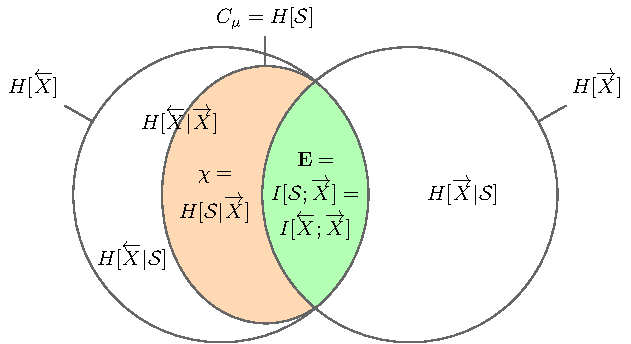
\includegraphics[scale = 1.0]{../chapter1/figures/tikz/3var_PastFutureS}
\caption{This highlights the crypticity $\PC$ in orange as the difference between the state information $\Cmu$ and the predictive information $\EE$. In this sense, crypticity can be thought of as `modeling overhead'.}
\label{fig:3var_PastFutureS}
\end{figure}

\subsection{Cryptic Order}
As the crypticity is a newly defined quantity, it is natural to attempt to tease it apart in ways similar to quantities we have dealt with in the past. The crypticity can be interpreted as the state-based companion information to the predicive information, $\EE$. That said, the primary dissection tool used to understand processes by thinking about their predictive information has been the Markov order. The Markov order describes the length scale of the correlations among symbols that give rise to probabilistic conditional independence; this independence is another way of describing an optimal predictor.

To begin, it is useful to have a picture of what Markov order is in terms of our I-diagram. We can stratify the past in terms of the random variables $\{\MeasSymbol_{-1}^{1}, \MeasSymbol_{-2}^{2}, \MeasSymbol_{-3}^{3}, ...\}$. The intersection of this stratification with the future is shown in Fig.~\ref{fig:FoliationMarkov}. For the details as to why intersection with a stratification is allowed in this way, and for why it is also non-trivial, see App.~\ref{app:Venn}. One feature of \eMs\ is illustrated by the fact that an equivalent way of understanding Markov order is the depth of history required for determining the causal state. It is this which speaks to the fundamental nature of causal states, and which allows us to make the statement that the cryptic order is a `companion' order.

\begin{figure}[h!]
\centering
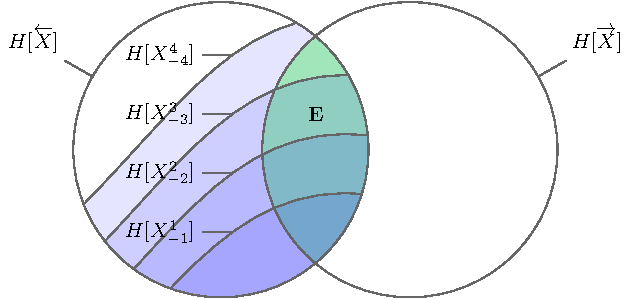
\includegraphics[scale = 1.2]{../chapter1/figures/tikz/FoliationMarkov}
\caption{An illustration of a process which is order-4 Markov. The past $H[\protect \Past]$ is shown as being stratified in the standard way. We can see that conditioning on the past 4 variables reduces as much uncertainty in the future as does conditioning on the entire past. Conditioning on only the past 3 variables, however, neglects the upper tip of the mutual information, $\EE=I[\protect\Past;\protect\Future]$.}
\label{fig:FoliationMarkov}
\end{figure}

\begin{figure}[h!]
\centering
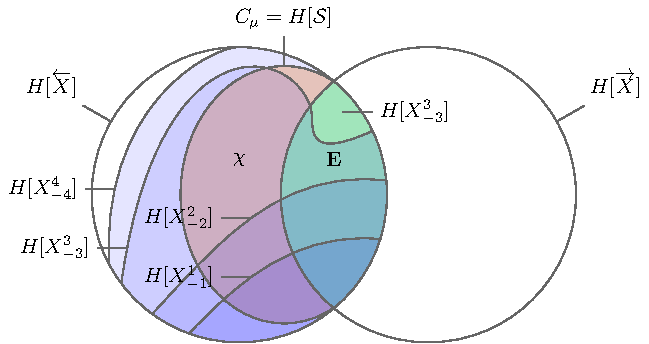
\includegraphics[scale = 1.2]{../chapter1/figures/tikz/FoliationCrypticReqk}
\caption{This is another illustration of an order-4 Markov process. The causal state has been added to the diagram and the boundaries made a little more curvy to anticipate future I-diagrams. Notice that in addition to the length 4 statistics being sufficient for capturing $\EE$, the same is true for capturing $\PC$ which is the remainder of $\Cmu$. In contrast, the length 3 statistics are insufficient for both $\EE$ and $\PC$. Being insufficient for $\EE$ is why the process is order-4 Markov. Being insufficient for $\PC$ is why the process is order-4 cryptic.}
\label{fig:FoliationCrypticReqk}
\end{figure}

Cryptic order is a new length scale introduced to characterize the way in which the information associated with crypticity is distributed in the process. We argue that the cryptic order is as fundamental to the nature of processes as the Markov order. It has a slightly different flavor in that it involves causal states, whereas Markov order can be defined without them. For an illustration as to how the cryptic and Markov orders can be different, see Fig.~\ref{fig:FoliationCryptic}. The cryptic order is the length scale appropriate for capturing the uncertainty in the causal state \emph{given the future}---it captures the crypticity.

\begin{figure}[h!]
\centering
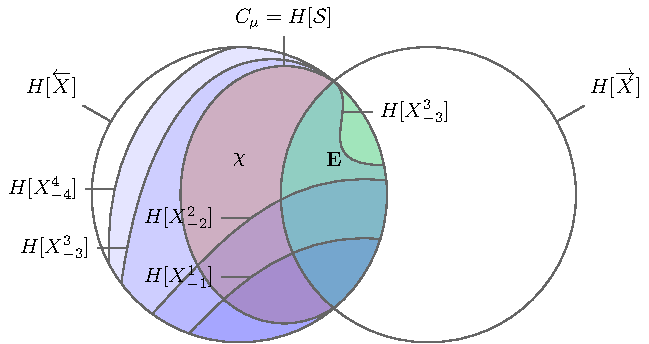
\includegraphics[scale = 1.2]{../chapter1/figures/tikz/FoliationCryptic}
\caption{An illustration of a process with differing cryptic and Markov orders. The Markov order is 4; this is the first history length which contains all of the predictive information. Notice that the length 3 history curves back again missing a portion of $\EE$. The cryptic order is 3 because although the length 3 history misses some portion of $\EE$, it does determine the causal state conditioned on the future. Note that $H[\MeasSymbol_{-3}^3]$ is labeled twice for clarity.}
\label{fig:FoliationCryptic}
\end{figure}

\begin{figure}[h!]
\centering
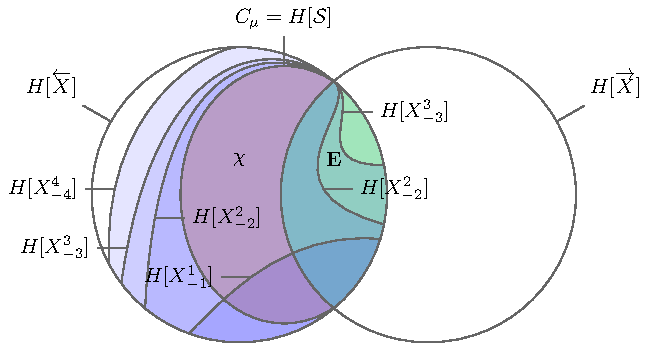
\includegraphics[scale = 1.2]{../chapter1/figures/tikz/FoliationCrypticRgegek}
\caption{The Markov and cryptic orders may differ by more than one. This is an instance where the Markov order is 4, yet the cryptic order is 2. Two entropies are labeled twice for clarity.}
\label{fig:FoliationCrypticRgegek}
\end{figure}

Properties of the crypticity and the cryptic order are the subjects of Ch.~\ref{ch.IACP}. This collection of definitions and proofs marks the beginning of a new and fundamental characterization of stochastic process. This characterization is thought to be fundamental as it is such a close analog to the Markov order. It is deemed impactful because, unlike the Markov order, it makes reference to states, something that the generically non-zero crypticity strongly suggests we do. Also, the states refered to are not any state, but causal states, and so the naturalness of the \eM\ in its ability to deliver quantities such as $\hmu$ and $\Cmu$ extends this naturalness to the cryptic order.


%%%%%%%
%\begin{figure}
%\caption{Scientia ex $\epsilon$-Machina}
%\end{figure}
%%%%%%%




%%%%%%%%%%%%%%%%%%%%%%%%%%%%%%%%%%%%%%%%%%%%%%%%%%%%%%%%%%%%%%%%%%%%%

\ifx\master\undefined% AUTOCOMPILE
% Allows for individual chapters to be compiled.

% Usage:
% \ifx\master\undefined% AUTOCOMPILE
% Allows for individual chapters to be compiled.

% Usage:
% \ifx\master\undefined% AUTOCOMPILE
% Allows for individual chapters to be compiled.

% Usage:
% \ifx\master\undefined\input{../settings/autocompile}\fi
% (place at start and end of chapter file)

\ifx\noprelim\undefined
    % first time included
    % input preamble files
    \input{../settings/phdsetup}

    \begin{document}
    \def\noprelim{}
\else
    % already included once
    % input post files

    \singlespacing
    \bibliographystyle{../bibliography/expanded}
    \bibliography{../bibliography/references}

    \end{document}
\fi\fi
% (place at start and end of chapter file)

\ifx\noprelim\undefined
    % first time included
    % input preamble files
    % [ USER VARIABLES ]

\def\PHDTITLE {Extensions of the Theory of Computational Mechanics}
\def\PHDAUTHOR{Evan Klose Friis}
\def\PHDSCHOOL{University of California, Davis}

\def\PHDMONTH {June}
\def\PHDYEAR  {2011}
\def\PHDDEPT {Physics}

\def\BSSCHOOL {University of California at San Diego}
\def\BSYEAR   {2005}

\def\PHDCOMMITTEEA{Professor John Conway}
\def\PHDCOMMITTEEB{Professor Robin Erbacher}
\def\PHDCOMMITTEEC{Professor Mani Tripathi}

% [ GLOBAL SETUP ]

\documentclass[letterpaper,oneside,11pt]{report}

\usepackage{calc}
\usepackage{breakcites}
\usepackage[newcommands]{ragged2e}

\usepackage[pdftex]{graphicx}
\usepackage{epstopdf}

%\usepackage{tikz}
%\usetikzlibrary{positioning} % [right=of ...]
%\usetikzlibrary{fit} % [fit= ...]

%\pgfdeclarelayer{background layer}
%\pgfdeclarelayer{foreground layer}
%\pgfsetlayers{background layer,main,foreground layer}

%\newenvironment{wrap}{\noindent\begin{minipage}[t]{\linewidth}\vspace{-0.5\normalbaselineskip}\centering}{\vspace{0.5\normalbaselineskip}\end{minipage}}

%% [Venn diagram environment]
%\newenvironment{venn2}
%{\begin{tikzpicture} [every pin/.style={text=black, text opacity=1.0, pin distance=0.5cm, pin edge={black!60, semithick}},
%% define a new style 'venn'
%venn/.style={circle, draw=black!60, semithick, minimum size = 4cm}]
%
%% create circle and give it external (pin) label
%\node[venn] (X) at (-1,0) [pin={150:$H[X]$}] {};
%\node[venn] (Y) at (1,0) [pin={30:$H[Y]$}] {};
%
%% place labels of the atoms by hand
%\node at (-1.9,0) {$H[X|Y]$};
%\node at (1.9,0) {$H[Y|X]$};
%\node at (0,0) {$I[X;Y]$};}
%{\end{tikzpicture}}

%\newcommand{\wrapmath}[1]{\begin{wrap}\begin{tikzpicture}[every node/.style={inner ysep=0ex, inner xsep=0em}]\node[] {$\displaystyle\begin{aligned} #1\end{aligned}$};\end{tikzpicture}\end{wrap}}

\renewenvironment{abstract}{\chapter*{Abstract}}{}
\renewcommand{\bibname}{Bibliography}
\renewcommand{\contentsname}{Table of Contents}

\makeatletter
\renewcommand{\@biblabel}[1]{\textsc{#1}}
\makeatother

% [ FONT SETTINGS ]

\usepackage[tbtags, intlimits, namelimits]{amsmath}
\usepackage[adobe-utopia]{mathdesign}

\DeclareSymbolFont{pazomath}{OMS}{zplm}{m}{n}
\DeclareSymbolFontAlphabet{\mathcal}{pazomath}
\SetMathAlphabet\mathcal{bold}{OMS}{zplm}{b}{n}

\SetSymbolFont{largesymbols}{normal}{OMX}{zplm}{m}{n}
\SetSymbolFont{largesymbols}{bold}{OMX}{zplm}{m}{n}
\SetSymbolFont{symbols}{normal}{OMS}{zplm}{m}{n}
\SetSymbolFont{symbols}{bold}{OMS}{zplm}{b}{n}

\renewcommand{\sfdefault}{phv}
\renewcommand{\ttdefault}{fvm}

\widowpenalty 8000
\clubpenalty  8000

% [ PAGE LAYOUT ]
\usepackage{geometry}
\geometry{lmargin = 1.5in}
\geometry{rmargin = 1.0in}
\geometry{tmargin = 1.0in}
\geometry{bmargin = 1.0in}

% [ PDF SETTINGS ]

\usepackage[final]{hyperref}
\hypersetup{breaklinks  = true}
\hypersetup{colorlinks  = true}
\hypersetup{linktocpage = false}
\hypersetup{linkcolor   = blue}
\hypersetup{citecolor   = green}
\hypersetup{urlcolor    = black}
\hypersetup{plainpages  = false}
\hypersetup{pageanchor  = true}
\hypersetup{pdfauthor   = {\PHDAUTHOR}}
\hypersetup{pdftitle    = {\PHDTITLE}}
\hypersetup{pdfsubject  = {Dissertation, \PHDSCHOOL}}
\urlstyle{same}

% [ LETTER SPACING ]

\usepackage[final]{microtype}
\microtypesetup{protrusion=compatibility}
\microtypesetup{expansion=false}

\newcommand{\upper}[1]{\MakeUppercase{#1}}
\let\lsscshape\scshape

\ifcase\pdfoutput\else\microtypesetup{letterspace=15}
\renewcommand{\scshape}{\lsscshape\lsstyle}
\renewcommand{\upper}[1]{\textls[50]{\MakeUppercase{#1}}}\fi

% [ LINE SPACING ]

\usepackage[doublespacing]{setspace}
\renewcommand{\displayskipstretch}{0.0}

\setlength{\parskip   }{0em}
\setlength{\parindent }{2em}

% [ TABLE FORMATTING ]

\usepackage{booktabs}
\setlength{\heavyrulewidth}{1.5\arrayrulewidth}
\setlength{\lightrulewidth}{1.0\arrayrulewidth}
\setlength{\doublerulesep }{2.0\arrayrulewidth}

% [ SECTION FORMATTING ]

\usepackage[largestsep,nobottomtitles*]{titlesec}
\renewcommand{\bottomtitlespace}{0.75in}

\titleformat{\chapter}[display]{\bfseries\huge\singlespacing}{\filleft\textsc{\LARGE \chaptertitlename\ \thechapter}}{-0.2ex}{\titlerule[3pt]\vspace{0.2ex}}[]

\titleformat{\section}{\LARGE}{\S\thesection\hspace{0.5em}}{0ex}{}
\titleformat{\subsection}{\Large}{\S\thesubsection\hspace{0.5em}}{0ex}{}
\titleformat{\subsubsection}{\large}{\thesubsubsection\hspace{0.5em}}{0ex}{}

\titlespacing*{\chapter}{0em}{6ex}{4ex plus 2ex minus 0ex}
\titlespacing*{\section}{0em}{2ex plus 3ex minus 1ex}{0.5ex plus 0.5ex minus 0.5ex}
\titlespacing*{\subsection}{0ex}{2ex plus 3ex minus 1ex}{0ex}
\titlespacing*{\subsubsection}{0ex}{2ex plus 0ex minus 1ex}{0ex}

% [ HEADER SETTINGS ]

\usepackage{fancyhdr}

\setlength{\headheight}{\normalbaselineskip}
\setlength{\footskip  }{0.5in}
\setlength{\headsep   }{0.5in-\headheight}

\fancyheadoffset[R]{0.5in}
\renewcommand{\headrulewidth}{0pt}
\renewcommand{\footrulewidth}{0pt}

\newcommand{\pagebox}{\parbox[r][\headheight][t]{0.5in}{\hspace\fill\thepage}}

\newcommand{\prelimheaders}{\ifx\prelim\undefined\renewcommand{\thepage}{\textit{\roman{page}}}\fancypagestyle{plain}{\fancyhf{}\fancyfoot[L]{\makebox[\textwidth-0.5in]{\thepage}}}\pagestyle{plain}\def\prelim{}\fi}

\newcommand{\normalheaders}{\renewcommand{\thepage}{\arabic{page}}\fancypagestyle{plain}{\fancyhf{}\fancyhead[R]{\pagebox}}\pagestyle{plain}}

\normalheaders{}

% [ CUSTOM COMMANDS ]

\newcommand{\signaturebox}[1]{\multicolumn{1}{p{4in}}{\vspace{3ex}}\\\midrule #1\\}

%\input{../includes/cmechabbrev}

% [some math stuff - maybe stick in sep file]
\usepackage{amsthm}
\usepackage{amscd}
\theoremstyle{plain}    \newtheorem{Lem}{Lemma}
\theoremstyle{plain}    \newtheorem*{ProLem}{Proof}
\theoremstyle{plain} 	\newtheorem{Cor}{Corollary}
\theoremstyle{plain} 	\newtheorem*{ProCor}{Proof}
\theoremstyle{plain} 	\newtheorem{The}{Theorem}
\theoremstyle{plain} 	\newtheorem*{ProThe}{Proof}
\theoremstyle{plain} 	\newtheorem{Prop}{Proposition}
\theoremstyle{plain} 	\newtheorem*{ProProp}{Proof}
\theoremstyle{plain} 	\newtheorem*{Conj}{Conjecture}
\theoremstyle{plain}	\newtheorem*{Rem}{Remark}
\theoremstyle{plain}	\newtheorem*{Def}{Definition} 
\theoremstyle{plain}	\newtheorem*{Not}{Notation}

% [uniform figure scaling - maybe this is not a good idea]
\def\figscale{.7}
\def\lscale{1.0}

% [FIX ME! - red makes it easier to spot]
\newcommand{\FIX}[1]{\textbf{\textcolor{red}{#1}}}


    \begin{document}
    \def\noprelim{}
\else
    % already included once
    % input post files

    \singlespacing
    \bibliographystyle{../bibliography/expanded}
    \bibliography{../bibliography/references}

    \end{document}
\fi\fi
% (place at start and end of chapter file)

\ifx\noprelim\undefined
    % first time included
    % input preamble files
    % [ USER VARIABLES ]

\def\PHDTITLE {Extensions of the Theory of Computational Mechanics}
\def\PHDAUTHOR{Evan Klose Friis}
\def\PHDSCHOOL{University of California, Davis}

\def\PHDMONTH {June}
\def\PHDYEAR  {2011}
\def\PHDDEPT {Physics}

\def\BSSCHOOL {University of California at San Diego}
\def\BSYEAR   {2005}

\def\PHDCOMMITTEEA{Professor John Conway}
\def\PHDCOMMITTEEB{Professor Robin Erbacher}
\def\PHDCOMMITTEEC{Professor Mani Tripathi}

% [ GLOBAL SETUP ]

\documentclass[letterpaper,oneside,11pt]{report}

\usepackage{calc}
\usepackage{breakcites}
\usepackage[newcommands]{ragged2e}

\usepackage[pdftex]{graphicx}
\usepackage{epstopdf}

%\usepackage{tikz}
%\usetikzlibrary{positioning} % [right=of ...]
%\usetikzlibrary{fit} % [fit= ...]

%\pgfdeclarelayer{background layer}
%\pgfdeclarelayer{foreground layer}
%\pgfsetlayers{background layer,main,foreground layer}

%\newenvironment{wrap}{\noindent\begin{minipage}[t]{\linewidth}\vspace{-0.5\normalbaselineskip}\centering}{\vspace{0.5\normalbaselineskip}\end{minipage}}

%% [Venn diagram environment]
%\newenvironment{venn2}
%{\begin{tikzpicture} [every pin/.style={text=black, text opacity=1.0, pin distance=0.5cm, pin edge={black!60, semithick}},
%% define a new style 'venn'
%venn/.style={circle, draw=black!60, semithick, minimum size = 4cm}]
%
%% create circle and give it external (pin) label
%\node[venn] (X) at (-1,0) [pin={150:$H[X]$}] {};
%\node[venn] (Y) at (1,0) [pin={30:$H[Y]$}] {};
%
%% place labels of the atoms by hand
%\node at (-1.9,0) {$H[X|Y]$};
%\node at (1.9,0) {$H[Y|X]$};
%\node at (0,0) {$I[X;Y]$};}
%{\end{tikzpicture}}

%\newcommand{\wrapmath}[1]{\begin{wrap}\begin{tikzpicture}[every node/.style={inner ysep=0ex, inner xsep=0em}]\node[] {$\displaystyle\begin{aligned} #1\end{aligned}$};\end{tikzpicture}\end{wrap}}

\renewenvironment{abstract}{\chapter*{Abstract}}{}
\renewcommand{\bibname}{Bibliography}
\renewcommand{\contentsname}{Table of Contents}

\makeatletter
\renewcommand{\@biblabel}[1]{\textsc{#1}}
\makeatother

% [ FONT SETTINGS ]

\usepackage[tbtags, intlimits, namelimits]{amsmath}
\usepackage[adobe-utopia]{mathdesign}

\DeclareSymbolFont{pazomath}{OMS}{zplm}{m}{n}
\DeclareSymbolFontAlphabet{\mathcal}{pazomath}
\SetMathAlphabet\mathcal{bold}{OMS}{zplm}{b}{n}

\SetSymbolFont{largesymbols}{normal}{OMX}{zplm}{m}{n}
\SetSymbolFont{largesymbols}{bold}{OMX}{zplm}{m}{n}
\SetSymbolFont{symbols}{normal}{OMS}{zplm}{m}{n}
\SetSymbolFont{symbols}{bold}{OMS}{zplm}{b}{n}

\renewcommand{\sfdefault}{phv}
\renewcommand{\ttdefault}{fvm}

\widowpenalty 8000
\clubpenalty  8000

% [ PAGE LAYOUT ]
\usepackage{geometry}
\geometry{lmargin = 1.5in}
\geometry{rmargin = 1.0in}
\geometry{tmargin = 1.0in}
\geometry{bmargin = 1.0in}

% [ PDF SETTINGS ]

\usepackage[final]{hyperref}
\hypersetup{breaklinks  = true}
\hypersetup{colorlinks  = true}
\hypersetup{linktocpage = false}
\hypersetup{linkcolor   = blue}
\hypersetup{citecolor   = green}
\hypersetup{urlcolor    = black}
\hypersetup{plainpages  = false}
\hypersetup{pageanchor  = true}
\hypersetup{pdfauthor   = {\PHDAUTHOR}}
\hypersetup{pdftitle    = {\PHDTITLE}}
\hypersetup{pdfsubject  = {Dissertation, \PHDSCHOOL}}
\urlstyle{same}

% [ LETTER SPACING ]

\usepackage[final]{microtype}
\microtypesetup{protrusion=compatibility}
\microtypesetup{expansion=false}

\newcommand{\upper}[1]{\MakeUppercase{#1}}
\let\lsscshape\scshape

\ifcase\pdfoutput\else\microtypesetup{letterspace=15}
\renewcommand{\scshape}{\lsscshape\lsstyle}
\renewcommand{\upper}[1]{\textls[50]{\MakeUppercase{#1}}}\fi

% [ LINE SPACING ]

\usepackage[doublespacing]{setspace}
\renewcommand{\displayskipstretch}{0.0}

\setlength{\parskip   }{0em}
\setlength{\parindent }{2em}

% [ TABLE FORMATTING ]

\usepackage{booktabs}
\setlength{\heavyrulewidth}{1.5\arrayrulewidth}
\setlength{\lightrulewidth}{1.0\arrayrulewidth}
\setlength{\doublerulesep }{2.0\arrayrulewidth}

% [ SECTION FORMATTING ]

\usepackage[largestsep,nobottomtitles*]{titlesec}
\renewcommand{\bottomtitlespace}{0.75in}

\titleformat{\chapter}[display]{\bfseries\huge\singlespacing}{\filleft\textsc{\LARGE \chaptertitlename\ \thechapter}}{-0.2ex}{\titlerule[3pt]\vspace{0.2ex}}[]

\titleformat{\section}{\LARGE}{\S\thesection\hspace{0.5em}}{0ex}{}
\titleformat{\subsection}{\Large}{\S\thesubsection\hspace{0.5em}}{0ex}{}
\titleformat{\subsubsection}{\large}{\thesubsubsection\hspace{0.5em}}{0ex}{}

\titlespacing*{\chapter}{0em}{6ex}{4ex plus 2ex minus 0ex}
\titlespacing*{\section}{0em}{2ex plus 3ex minus 1ex}{0.5ex plus 0.5ex minus 0.5ex}
\titlespacing*{\subsection}{0ex}{2ex plus 3ex minus 1ex}{0ex}
\titlespacing*{\subsubsection}{0ex}{2ex plus 0ex minus 1ex}{0ex}

% [ HEADER SETTINGS ]

\usepackage{fancyhdr}

\setlength{\headheight}{\normalbaselineskip}
\setlength{\footskip  }{0.5in}
\setlength{\headsep   }{0.5in-\headheight}

\fancyheadoffset[R]{0.5in}
\renewcommand{\headrulewidth}{0pt}
\renewcommand{\footrulewidth}{0pt}

\newcommand{\pagebox}{\parbox[r][\headheight][t]{0.5in}{\hspace\fill\thepage}}

\newcommand{\prelimheaders}{\ifx\prelim\undefined\renewcommand{\thepage}{\textit{\roman{page}}}\fancypagestyle{plain}{\fancyhf{}\fancyfoot[L]{\makebox[\textwidth-0.5in]{\thepage}}}\pagestyle{plain}\def\prelim{}\fi}

\newcommand{\normalheaders}{\renewcommand{\thepage}{\arabic{page}}\fancypagestyle{plain}{\fancyhf{}\fancyhead[R]{\pagebox}}\pagestyle{plain}}

\normalheaders{}

% [ CUSTOM COMMANDS ]

\newcommand{\signaturebox}[1]{\multicolumn{1}{p{4in}}{\vspace{3ex}}\\\midrule #1\\}

%%%% macros fro standard references
%\eqref provided by amsmath
\newcommand{\figref}[1]{Fig.~\ref{#1}}
\newcommand{\tableref}[1]{Table~\ref{#1}}
\newcommand{\refcite}[1]{Ref.~\cite{#1}}

% Abbreviations from CMPPSS:

\newcommand{\eM}     {\mbox{$\epsilon$-machine}}
\newcommand{\eMs}    {\mbox{$\epsilon$-machines}}
\newcommand{\EM}     {\mbox{$\epsilon$-Machine}}
\newcommand{\EMs}    {\mbox{$\epsilon$-Machines}}
\newcommand{\eT}     {\mbox{$\epsilon$-transducer}}
\newcommand{\eTs}    {\mbox{$\epsilon$-transducers}}
\newcommand{\ET}     {\mbox{$\epsilon$-Transducer}}
\newcommand{\ETs}    {\mbox{$\epsilon$-Transducers}}

% Processes and sequences

\newcommand{\Process}{\mathcal{P}}

\newcommand{\ProbMach}{\Prob_{\mathrm{M}}}
\newcommand{\Lmax}   { {L_{\mathrm{max}}}}
\newcommand{\MeasAlphabet}	{\mathcal{A}}
% Original
%\newcommand{\MeasSymbol}   { {S} }
%\newcommand{\meassymbol}   { {s} }
% New symbol
\newcommand{\MeasSymbol}   { {X} }
\newcommand{\meassymbol}   { {x} }
\newcommand{\BiInfinity}	{ \overleftrightarrow {\MeasSymbol} }
\newcommand{\biinfinity}	{ \overleftrightarrow {\meassymbol} }
\newcommand{\Past}	{ \overleftarrow {\MeasSymbol} }
\newcommand{\past}	{ {\overleftarrow {\meassymbol}} }
\newcommand{\pastprime}	{ {\past}^{\prime}}
\newcommand{\Future}	{ \overrightarrow{\MeasSymbol} }
\newcommand{\future}	{ \overrightarrow{\meassymbol} }
\newcommand{\futureprime}	{ {\future}^{\prime}}
\newcommand{\PastPrime}	{ {\Past}^{\prime}}
\newcommand{\FuturePrime}	{ {\overrightarrow{\meassymbol}}^\prime }
\newcommand{\PastDblPrime}	{ {\overleftarrow{\meassymbol}}^{\prime\prime} }
\newcommand{\FutureDblPrime}	{ {\overrightarrow{\meassymbol}}^{\prime\prime} }
\newcommand{\pastL}	{ {\overleftarrow {\meassymbol}}{}^L }
\newcommand{\PastL}	{ {\overleftarrow {\MeasSymbol}}{}^L }
\newcommand{\PastLt}	{ {\overleftarrow {\MeasSymbol}}_t^L }
\newcommand{\PastLLessOne}	{ {\overleftarrow {\MeasSymbol}}^{L-1} }
\newcommand{\futureL}	{ {\overrightarrow{\meassymbol}}{}^L }
\newcommand{\FutureL}	{ {\overrightarrow{\MeasSymbol}}{}^L }
\newcommand{\FutureLt}	{ {\overrightarrow{\MeasSymbol}}_t^L }
\newcommand{\FutureLLessOne}	{ {\overrightarrow{\MeasSymbol}}^{L-1} }
\newcommand{\pastLprime}	{ {\overleftarrow {\meassymbol}}^{L^\prime} }
\newcommand{\futureLprime}	{ {\overrightarrow{\meassymbol}}^{L^\prime} }
\newcommand{\AllPasts}	{ { \overleftarrow {\rm {\bf \MeasSymbol}} } }
\newcommand{\AllFutures}	{ \overrightarrow {\rm {\bf \MeasSymbol}} }
\newcommand{\FutureSet}	{ \overrightarrow{\bf \MeasSymbol}}

% Causal states and epsilon-machines
\newcommand{\CausalState}	{ \mathcal{S} }
\newcommand{\CausalStatePrime}	{ {\CausalState}^{\prime}}
\newcommand{\causalstate}	{ \sigma }
\newcommand{\CausalStateSet}	{ \boldsymbol{\CausalState} }
\newcommand{\AlternateState}	{ \mathcal{R} }
\newcommand{\AlternateStatePrime}	{ {\cal R}^{\prime} }
\newcommand{\alternatestate}	{ \rho }
\newcommand{\alternatestateprime}	{ {\rho^{\prime}} }
\newcommand{\AlternateStateSet}	{ \boldsymbol{\AlternateState} }
\newcommand{\PrescientState}	{ \widehat{\AlternateState} }
\newcommand{\prescientstate}	{ \widehat{\alternatestate} }
\newcommand{\PrescientStateSet}	{ \boldsymbol{\PrescientState}}
\newcommand{\CausalEquivalence}	{ {\sim}_{\epsilon} }
\newcommand{\CausalEquivalenceNot}	{ {\not \sim}_{\epsilon}}

\newcommand{\NonCausalEquivalence}	{ {\sim}_{\eta} }
\newcommand{\NextObservable}	{ {\overrightarrow {\MeasSymbol}}^1 }
\newcommand{\LastObservable}	{ {\overleftarrow {\MeasSymbol}}^1 }
%\newcommand{\Prob}		{ {\rm P}}
\newcommand{\Prob}      {\Pr} % use standard command
\newcommand{\ProbAnd}	{ {,\;} }
\newcommand{\LLimit}	{ {L \rightarrow \infty}}
\newcommand{\Cmu}		{C_\mu}
\newcommand{\hmu}		{h_\mu}
\newcommand{\EE}		{{\bf E}}
\newcommand{\Measurable}{{\bf \mu}}

% Process Crypticity
\newcommand{\PC}		{\chi}
\newcommand{\FuturePC}		{\PC^+}
\newcommand{\PastPC}		{\PC^-}
% Causal Irreversibility
\newcommand{\CI}		{\Xi}
\newcommand{\ReverseMap}	{r}
\newcommand{\ForwardMap}	{f}

% Abbreviations from IB:
% None that aren't already in CMPPSS

% Abbreviations from Extensive Estimation:
\newcommand{\EstCausalState}	{\widehat{\CausalState}}
\newcommand{\estcausalstate}	{\widehat{\causalstate}}
\newcommand{\EstCausalStateSet}	{\boldsymbol{\EstCausalState}}
\newcommand{\EstCausalFunc}	{\widehat{\epsilon}}
\newcommand{\EstCmu}		{\widehat{\Cmu}}
\newcommand{\PastLOne}	{{\Past}^{L+1}}
\newcommand{\pastLOne}	{{\past}^{L+1}}

% Abbreviations from $\epsilon$-Transducers:
\newcommand{\InAlphabet}	{ \mathcal{A}}
\newcommand{\insymbol}		{ a}
\newcommand{\OutAlphabet}	{ \mathcal{B}}
\newcommand{\outsymbol}		{ b}
\newcommand{\InputSimple}	{ X}
\newcommand{\inputsimple}	{ x}
\newcommand{\BottleneckVar}	{\tilde{\InputSimple}}
\newcommand{\bottleneckvar}	{\tilde{\inputsimple}}
\newcommand{\InputSpace}	{ \mathbf{\InputSimple}}
\newcommand{\InputBi}	{ \overleftrightarrow {\InputSimple} }
\newcommand{\inputbi}	{ \overleftrightarrow {\inputsimple} }
\newcommand{\InputPast}	{ \overleftarrow {\InputSimple} }
\newcommand{\inputpast}	{ \overleftarrow {\inputsimple} }
\newcommand{\InputFuture}	{ \overrightarrow {\InputSimple} }
\newcommand{\inputfuture}	{ \overrightarrow {\inputsimple} }
\newcommand{\NextInput}	{ {{\InputFuture}^{1}}}
\newcommand{\NextOutput}	{ {\OutputFuture}^{1}}
\newcommand{\OutputSimple}	{ Y}
\newcommand{\outputsimple}	{ y}
\newcommand{\OutputSpace}	{ \mathbf{\OutputSimple}}
\newcommand{\OutputBi}	{ \overleftrightarrow{\OutputSimple} }
\newcommand{\outputbi}	{ \overleftrightarrow{\outputsimple} }
\newcommand{\OutputPast}	{ \overleftarrow{\OutputSimple} }
\newcommand{\outputpast}	{ \overleftarrow{\outputsimple} }
\newcommand{\OutputFuture}	{ \overrightarrow{\OutputSimple} }
\newcommand{\outputfuture}	{ \overrightarrow{\outputsimple} }
\newcommand{\OutputL}	{ {\OutputFuture}^L}
\newcommand{\outputL}	{ {\outputfuture}^L}
\newcommand{\InputLLessOne}	{ {\InputFuture}^{L-1}}
\newcommand{\inputLlessone}	{ {\inputufutre}^{L-1}}
\newcommand{\OutputPastLLessOne}	{{\OutputPast}^{L-1}_{-1}}
\newcommand{\outputpastLlessone}	{{\outputpast}^{L-1}}
\newcommand{\OutputPastLessOne}	{{\OutputPast}_{-1}}
\newcommand{\outputpastlessone}	{{\outputpast}_{-1}}
\newcommand{\OutputPastL}	{{\OutputPast}^{L}}
\newcommand{\OutputLPlusOne}	{ {\OutputFuture}^{L+1}}
\newcommand{\outputLplusone}	{ {\outputfutre}^{L+1}}
\newcommand{\InputPastL}	{{\InputPast}^{L}}
\newcommand{\inputpastL}	{{\inputpast}^{L}}
\newcommand{\JointPast}	{{(\InputPast,\OutputPast)}}
\newcommand{\jointpast}	{{(\inputpast,\outputpast)}}
\newcommand{\jointpastone}	{{(\inputpast_1,\outputpast_1)}}
\newcommand{\jointpasttwo}	{{(\inputpast_2,\outputpast_2)}}
\newcommand{\jointpastprime} {{({\inputpast}^{\prime},{\outputpast}^{\prime})}}
\newcommand{\NextJoint}	{{(\NextInput,\NextOutput)}}
\newcommand{\nextjoint}	{{(\insymbol,\outsymbol)}}
\newcommand{\AllInputPasts}	{ { \overleftarrow {\rm \InputSpace}}}
\newcommand{\AllOutputPasts}	{ {\overleftarrow {\rm \OutputSpace}}}
\newcommand{\DetCausalState}	{ {{\cal S}_D }}
\newcommand{\detcausalstate}	{ {{\sigma}_D} }
\newcommand{\DetCausalStateSet}	{ \boldsymbol{{\CausalState}_D}}
\newcommand{\DetCausalEquivalence}	{ {\sim}_{{\epsilon}_{D}}}
\newcommand{\PrescientEquivalence}	{ {\sim}_{\widehat{\eta}}}
\newcommand{\FeedbackCausalState}	{ \mathcal{F}}
\newcommand{\feedbackcausalstate}	{ \phi}
\newcommand{\FeedbackCausalStateSet}	{ \mathbf{\FeedbackCausalState}}
\newcommand{\JointCausalState}		{ \mathcal{J}}
\newcommand{\JointCausalStateSet}	{ \mathbf{\JointCausalState}}
\newcommand{\UtilityFunctional}	{ {\mathcal{L}}}
\newcommand{\NatureState}	{ {\Omega}}
\newcommand{\naturestate}	{ {\omega}}
\newcommand{\NatureStateSpace}	{ {\mathbf{\NatureState}}}
\newcommand{\AnAction}	{ {A}}
\newcommand{\anaction}	{ {a}}
\newcommand{\ActionSpace}	{ {\mathbf{\AnAction}}}

% Abbreviations from RURO:
\newcommand{\InfoGain}[2] { \mathcal{D} \left( {#1} || {#2} \right) }

% Abbreviations from Upper Bound:
\newcommand{\lcm}	{{\rm lcm}}
% Double-check that this isn't in the math set already!

% Abbreviations from Emergence in Space
\newcommand{\ProcessAlphabet}	{\MeasAlphabet}
\newcommand{\ProbEst}			{ {\widehat{\Prob}_N}}
\newcommand{\STRegion}			{ {\mathrm K}}
\newcommand{\STRegionVariable}		{ K}
\newcommand{\stregionvariable}		{ k}
\newcommand{\GlobalPast}		{ \overleftarrow{G}} 
\newcommand{\globalpast}		{ \overleftarrow{g}} 
\newcommand{\GlobalFuture}		{ \overrightarrow{G}}
\newcommand{\globalfuture}		{ \overrightarrow{g}}
\newcommand{\GlobalState}		{ \mathcal{G}}
\newcommand{\globalstate}		{ \gamma}
\newcommand{\GlobalStateSet}		{ {\mathbf \GlobalState}}
\newcommand{\LocalPast}			{ \overleftarrow{L}} 
\newcommand{\localpast}			{ \overleftarrow{l}}
\newcommand{\AllLocalPasts}		{ \mathbf{\LocalPast}}
\newcommand{\LocalPastRegion}		{ \overleftarrow{\mathrm L}}
\newcommand{\LocalFuture}		{ \overrightarrow{L}}
\newcommand{\localfuture}		{ \overrightarrow{l}}
\newcommand{\LocalFutureRegion}		{ \overrightarrow{\mathrm L}}
\newcommand{\LocalState}		{ \mathcal{L}}
\newcommand{\localstate}		{ \lambda}
\newcommand{\LocalStateSet}		{ {\mathbf \LocalState}}
\newcommand{\PatchPast}			{ \overleftarrow{P}}
\newcommand{\patchpast}			{ \overleftarrow{p}}
\newcommand{\PatchPastRegion}		{ \overleftarrow{\mathrm P}}
\newcommand{\PatchFuture}		{ \overrightarrow{P}}
\newcommand{\patchfuture}		{ \overrightarrow{p}}
\newcommand{\PatchFutureRegion}		{ \overrightarrow{\mathrm P}}
\newcommand{\PatchState}		{ \mathcal{P}}
\newcommand{\patchstate}		{ \pi}
\newcommand{\PatchStateSet}		{ {\mathbf \PatchState}}
\newcommand{\LocalStatesInPatch}	{\vec{\LocalState}}
\newcommand{\localstatesinpatch}	{\vec{\localstate}}
\newcommand{\PointInstantX}		{ {\mathbf x}}
% Galles's original LaTeX for the cond. indep. symbol follows:
\newcommand{\compos}{\mbox{$~\underline{~\parallel~}~$}}
\newcommand{\ncompos}{\not\hspace{-.15in}\compos}
\newcommand{\indep}			{ \rotatebox{90}{$\models$}}
\newcommand{\nindep}	{\not\hspace{-.05in}\indep}
\newcommand{\LocalEE}	{{\EE}^{loc}}
\newcommand{\EEDensity}	{\overline{\LocalEE}}
\newcommand{\LocalCmu}	{{\Cmu}^{loc}}
\newcommand{\CmuDensity}	{\overline{\LocalCmu}}

%%%%%%%%%%% added by sasa
\newcommand{\FinPast}[1]	{ \overleftarrow {\MeasSymbol} \stackrel{{#1}}{}}
\newcommand{\finpast}[1]  	{ \overleftarrow {\meassymbol}  \stackrel{{#1}}{}}
\newcommand{\FinFuture}[1]		{ \overrightarrow{\MeasSymbol} \stackrel{{#1}}{}}
\newcommand{\finfuture}[1]		{ \overrightarrow{\meassymbol} \stackrel{{#1}}{}}

\newcommand{\Partition}	{ \AlternateState }
\newcommand{\partitionstate}	{ \alternatestate }
\newcommand{\PartitionSet}	{ \AlternateStateSet }
\newcommand{\Fdet}   { F_{\rm det} }

\newcommand{\Dkl}[2] { D_{\rm KL} \left( {#1} || {#2} \right) }

\newcommand{\Period}	{p}

% To take into account time direction
\newcommand{\forward}{+}
\newcommand{\reverse}{-}
%\newcommand{\forwardreverse}{\:\!\diamond} % \pm
\newcommand{\forwardreverse}{\pm} % \pm
\newcommand{\FutureProcess}	{ {\Process}^{\forward} }
\newcommand{\PastProcess}	{ {\Process}^{\reverse} }
\newcommand{\FutureCausalState}	{ {\CausalState}^{\forward} }
\newcommand{\futurecausalstate}	{ \sigma^{\forward} }
\newcommand{\altfuturecausalstate}	{ \sigma^{\forward\prime} }
\newcommand{\PastCausalState}	{ {\CausalState}^{\reverse} }
\newcommand{\pastcausalstate}	{ \sigma^{\reverse} }
\newcommand{\BiCausalState}		{ {\CausalState}^{\forwardreverse} }
\newcommand{\bicausalstate}		{ {\sigma}^{\forwardreverse} }
\newcommand{\FutureCausalStateSet}	{ {\CausalStateSet}^{\forward} }
\newcommand{\PastCausalStateSet}	{ {\CausalStateSet}^{\reverse} }
\newcommand{\BiCausalStateSet}	{ {\CausalStateSet}^{\forwardreverse} }
\newcommand{\eMachine}	{ M }
\newcommand{\FutureEM}	{ {\eMachine}^{\forward} }
\newcommand{\PastEM}	{ {\eMachine}^{\reverse} }
\newcommand{\BiEM}		{ {\eMachine}^{\forwardreverse} }
\newcommand{\BiEquiv}	{ {\sim}^{\forwardreverse} }
\newcommand{\Futurehmu}	{ h_\mu^{\forward} }
\newcommand{\Pasthmu}	{ h_\mu^{\reverse} }
\newcommand{\FutureCmu}	{ C_\mu^{\forward} }
\newcommand{\PastCmu}	{ C_\mu^{\reverse} }
\newcommand{\BiCmu}		{ C_\mu^{\forwardreverse} }
\newcommand{\FutureEps}	{ \epsilon^{\forward} }
\newcommand{\PastEps}	{ \epsilon^{\reverse} }
\newcommand{\BiEps}	{ \epsilon^{\forwardreverse} }
\newcommand{\FutureSim}	{ \sim^{\forward} }
\newcommand{\PastSim}	{ \sim^{\reverse} }
% Used arrows for awhile, more or less confusing?
%\newcommand{\FutureCausalState}	{ \overrightarrow{\CausalState} }
%\newcommand{\PastCausalState}	{ \overleftarrow{\CausalState} }
%\newcommand{\eMachine}	{ M }
%\newcommand{\FutureEM}	{ \overrightarrow{\eMachine} }
%\newcommand{\PastEM}	{ \overleftarrow{\eMachine} }
%\newcommand{\FutureCmu}	{ \overrightarrow{\Cmu} }
%\newcommand{\PastCmu}	{ \overleftarrow{\Cmu} }

%% time-reversing and mixed state presentation operators
\newcommand{\TR}{\mathcal{T}}
\newcommand{\MSP}{\mathcal{U}}
\newcommand{\one}{\mathbf{1}}

%% (cje)
%% Provide a command \ifpm which is true when \pm 
%% is meant to be understood as "+ or -". This is
%% different from the usage in TBA.
\newif\ifpm 
\edef\tempa{\forwardreverse}
\edef\tempb{\pm}
\ifx\tempa\tempb
   \pmfalse
\else
   \pmtrue  
\fi





% [some math stuff - maybe stick in sep file]
\usepackage{amsthm}
\usepackage{amscd}
\theoremstyle{plain}    \newtheorem{Lem}{Lemma}
\theoremstyle{plain}    \newtheorem*{ProLem}{Proof}
\theoremstyle{plain} 	\newtheorem{Cor}{Corollary}
\theoremstyle{plain} 	\newtheorem*{ProCor}{Proof}
\theoremstyle{plain} 	\newtheorem{The}{Theorem}
\theoremstyle{plain} 	\newtheorem*{ProThe}{Proof}
\theoremstyle{plain} 	\newtheorem{Prop}{Proposition}
\theoremstyle{plain} 	\newtheorem*{ProProp}{Proof}
\theoremstyle{plain} 	\newtheorem*{Conj}{Conjecture}
\theoremstyle{plain}	\newtheorem*{Rem}{Remark}
\theoremstyle{plain}	\newtheorem*{Def}{Definition} 
\theoremstyle{plain}	\newtheorem*{Not}{Notation}

% [uniform figure scaling - maybe this is not a good idea]
\def\figscale{.7}
\def\lscale{1.0}

% [FIX ME! - red makes it easier to spot]
\newcommand{\FIX}[1]{\textbf{\textcolor{red}{#1}}}


    \begin{document}
    \def\noprelim{}
\else
    % already included once
    % input post files

    \singlespacing
    \bibliographystyle{../bibliography/expanded}
    \bibliography{../bibliography/references}

    \end{document}
\fi\fi

